\documentclass{article}

% żeby użyć polskiego
\usepackage[T1]{fontenc}
\usepackage[polish]{babel}
\usepackage[utf8]{inputenc}

% żeby użyć matmy
\usepackage{amsmath}

% żeby pokazać kod
\usepackage{listings}

% żeby wklejać zdjęcia
\usepackage{graphicx}
\graphicspath{{../images/methods}}
% tabelki
\usepackage{array}

\usepackage{float}

\usepackage{url}



\title{Analiza skupień zestawu parametrów samochodów amerykańskich, europejskich i japońskich wyprodukowanych w latach 1970-1982}
\author{\fontsize{11}{13}\selectfont Jerzy Marczewski, \newline Dawid Rozumkiewicz, Wojciech Pietraszuk, Karol Hetmański, Przemysław Chachaj}
\author{
  Jerzy Marczewski\\
  \and
  Dawid Rozumkiewicz\\
  \and
  Wojciech Pietraszuk\\
  \and
  Karol Hetmański\\
  \and
  Przemysław Chachaj\\
}
\date{}
\begin{document}

\maketitle

\section{Streszczenie}
Przedmiotem badań są samochody pochodzenia amerykańskiego, europejskiego lub japońskiego wyprodukowane
w latach 1970-1982. Dane pobraliśmy z repozytorium na GitHub o nazwie ``exploratory-data-analysis-dataset-cars''
należącego do użytkownika o pseudonimie RodolfoViana. Dane składają się z nazwy samochodu i kilku podstawowych 
informacji o nich. Omawiane dane wczytaliśmy do do programu RStudio, a następnie dokonaliśmy obróbki danych.
Na początku usunęliśmy co drugi wiersz, ponieważ dane były tak obszerne, że prezentacja graficzna była dosyć nieczytelna.
Kolejnym krokiem było usunięcie wierszy, gdzie występowały znaki puste. Następnie usunęliśmy wiersze, gdzie powtarzały się 
nazwy samochodów, dzięki czemu te były unikalne, co sprawiło, że mogliśmy ich używać jako identyfikatorów. 
Obliczyliśmy statystyki opisowe. Wykorzystaliśmy metodę łokciową i silhouette w celu oszacowania optymalnej liczby klastrów, 
którą wykorzystaliśmy do metody k-średnich, Warda, complete, average i single. Potem użyliśmy techniki sieci Kohonena.


\section{Słowa kluczowe}
    \begin{itemize}
        \item klaster - zgrupowanie przestrzenne 
        \item klateryzacja - metoda klasyfikacji bez nadzoru (ang. usupervised learning), która grupuje elementy na względnie jednorodne klasy
        \item mpg - \textit{(ang. miles per gallon)} mile na galon
        \item objętość skokowa cylindra - różnica pomiędzy maksymalną a minimalną objętością cylindra
        \item objętość skokowa silnika - iloczyn objętości skokowej cylindra i liczby cylindrów
        \item hp - \textit{(ang. Horsepower)} konie mechaniczne
        \item metoda k-średnich - jest jednym z algorytmów stosowanym w analizie skupień, wykorzystywanym m.in. w kwantyzacji wektorowej
        \item metoda Warda -  jedna z aglomeracyjnych metod grupowania
        \item SOM - \textit{(ang. Self-organizing map)} sieć Kohonena 
        \item BMU - \textit{(ang. best matching unit)} najlepiej dopasowana jednostka
    \end{itemize}


\section{Wprowadzenie}
Okres 1970-1982 to ciekawy i ważny czas w motoryzacji. Na rynku występowała wtedy duża różnorodność, która niejako wymusza podział tego rynku na segmenty. Gdyby chcieć przyporządkować jednoznacznie każdy model do danego segmentu mogłoby się okazać, że może być z tym problem. W rozwiązaniu tego problemu z pomocą przychodzą nam różne metody analizy skupień. Mają one zastosowanie w fazie eksploracyjnej badań, gdy nie dysponujemy żadnymi hipotezami. Celem analizy skupień jest ułożenie obiektów w grupy w taki sposób, by obiekty należące do tej samej grupy były ze sobą jak najbardziej powiązane, a jednocześnie były jak najmniej związane z obiektami z pozostałych grup. Tym sposobem możemy uzyskać bardzo dobry podział modeli samochodów na różne grupy.
\section{Przedmiot badania}
    \subsection{Cel i zakres badania} 
    Badanie przeprowadzamy na podstawie danych różnych samochodów ze Stanów Zjednoczonych, Europy i Japonii. 
    Dane składają się z nazwy samochodów i ich parametrów technicznych.
    \newline\newline
    Naszym celem jest wykonanie analizy skupień samochodów. Badanie podzieli nam dane na klastry, na podstawie których będziemy mogli 
    wywnioskować, które samochody są do siebie podobne, a które się między sobą różnią. 
    \newline
    \subsection{(min. 1 cytowanie powiązane tematycznie i krótki opis co było badane)}
    ``W przypadku rynku samochodowego pozycjonowanie modelu samochodu w określonym segmencie nie zawsze w pełni oddaje faktyczny stan rzeczy. Nie istnieją bowiem w tym przypadku sztywne granice segmentów. Poszczególne segmenty raczej się zazębiają, powodując, że pewne modele znajdują się na pograniczu, a ich jednoznaczne przyporządkowanie jest mocno utrudnione.'' \newline- Bartłomiej Jefmański, Katedra Ekonometrii i Informatyki, Uniwersytet Ekonomiczny we Wrocławiu
    \newline\newline
    Badane były samochody pochodzenia europejskiego w różnych kategoriach cenowych.
    \subsection{Zmienne wybrane do analizy}
    Do analizy wybrano następujące cechy diagnostyczne:
    \begin{itemize}
        \item ${X_1}$ - mpg
        \item ${X_2}$ - liczba cylidnrów 
        \item ${X_3}$ - objętość skokowa silnika
        \item ${X_4}$ - hp
        \item ${X_5}$ - waga (podana w funtach)
        \item ${X_6}$ - przyspieszenie
        \item ${X_7}$ - model (rok modelowy auta wyrażony w dwóch ostanich cyfrach roku)
        \item ${X_8}$ - kraj pochodzenia (1 - Stany Zjednoczone, 2 - Europa, 3 - Japonia)
    \end{itemize}
    gdzie:
    \begin{itemize}
        \item ${X_1, X_2, X_3, X_4, X_6}$ to stymulanty
        \item ${X_5}$ to destymulanta
        \item ${X_7, X_8}$ to neutralne
    \end{itemize}
    
    
    \subsection{Wstępna analiza danych}
        \subsubsection*{Statystyki opisowe}
        Wyniki średniej, mediany, minimum, maksimum, odchylenia standardowego, skośności dla każdej z cech zaokrąglone do dwóch 
        miejsc po przeciunku:
        \begin{center}
            \begin{tabular}{ |c|c|c|c|c|c|c|c|c|c| } 
                \hline
                & ${X_1}$ & ${X_2}$ & ${X_3}$ & ${X_4}$ & ${X_5}$ & ${X_6}$ & ${X_7}$ & ${X_8}$ \\
                \hline
                średnia & 20.76  & 5.81 & 216.09 & 112.91 & 3139.32 & 15.31 & 74.35 & 1.46 \\
                \hline
                mediana & 19.2 & 6.0 & 225.0 & 100.0 & 3139.0 & 15.5 & 74.0 & 1.0 \\
                \hline
                min & 9 & 4 & 72 & 46 & 1613 & 9 & 70 & 1  \\
                \hline
                max & 43.1 & 8.0 & 455.0 & 230.0 & 5140.0 & 22.1 & 79.0 &  3.0  \\
                \hline
                odchylenie standardowe & 6.62 & 1.78 & 109.93 & 41.64 & 900.74 & 2.80 & 2.93 &  0.74  \\
                \hline
                skośność & 0.71 & 0.18 & 0.34 & 0.79 & 0.24 & 0.06 & 0.04 &  1.21 \\
                \hline
            \end{tabular}
        \end{center}
        \subsubsection*{Podstawowa wizualizacja danych}
            \begin{figure}[H]
                \caption{Wykres pudełkowy przed standaryzacją}
                \centering
                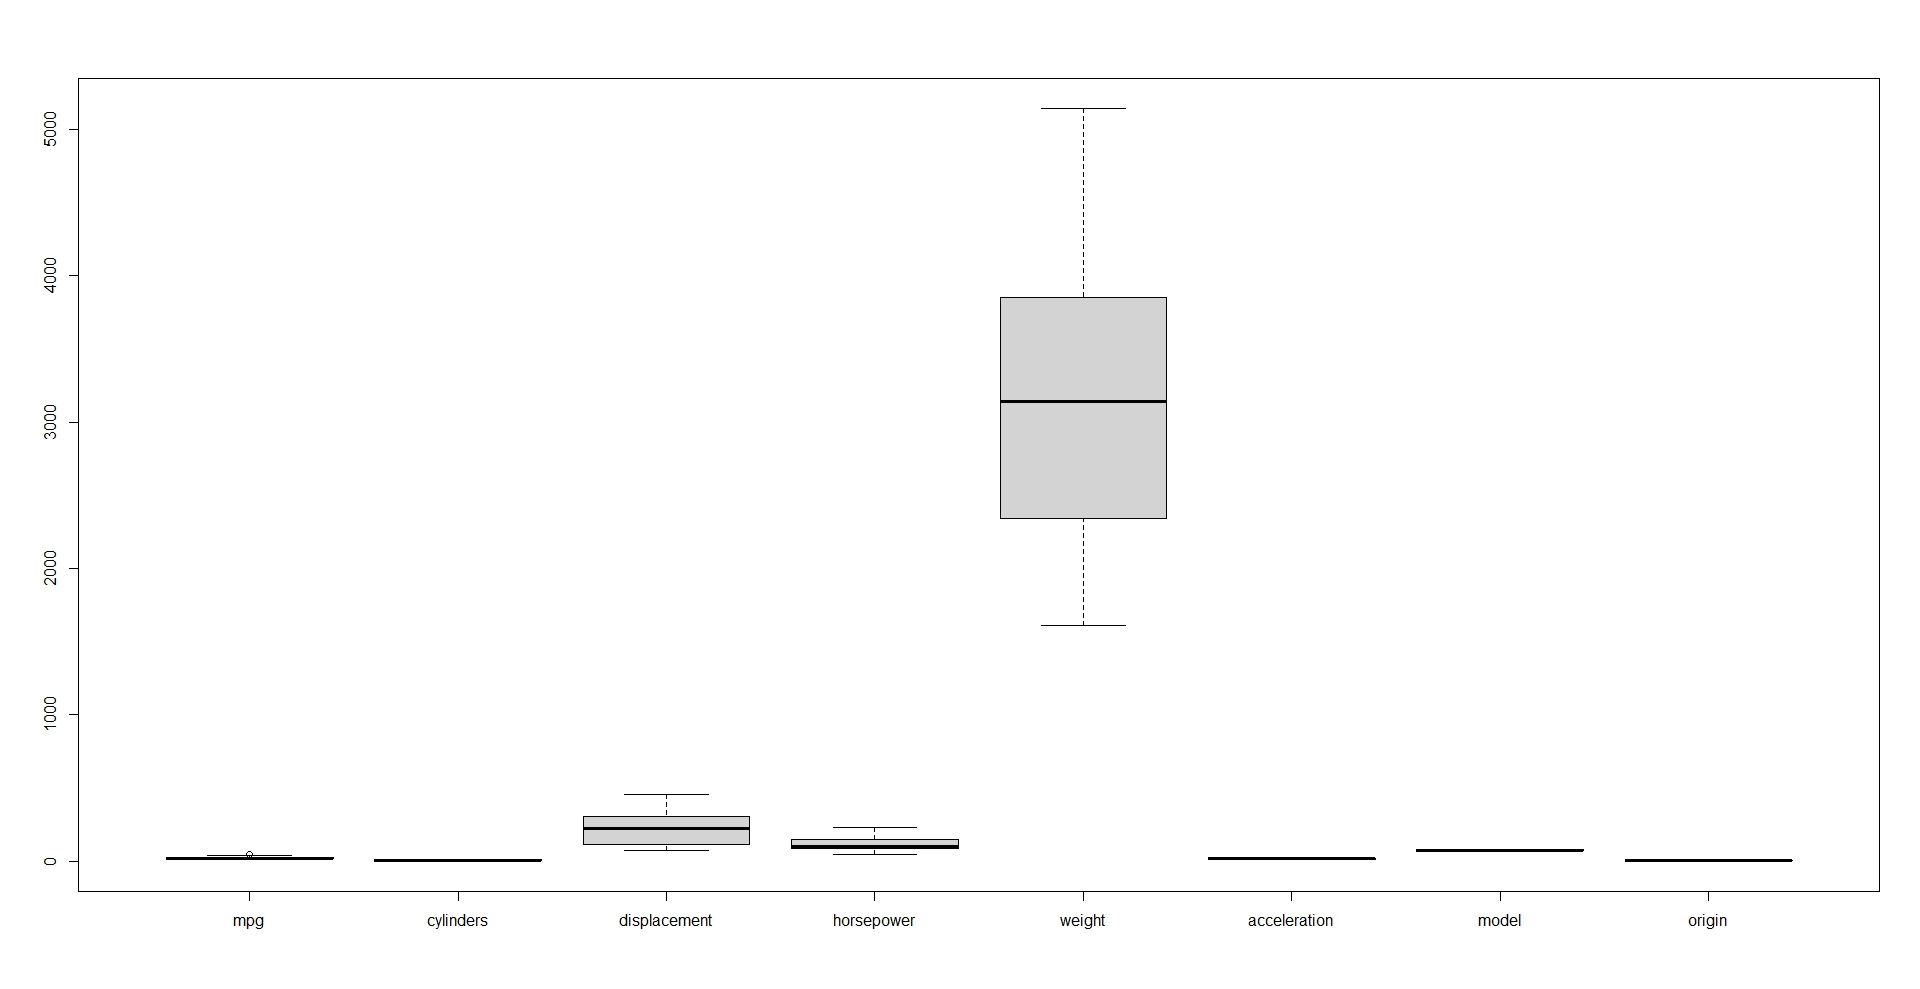
\includegraphics[width=\textwidth]{../boxplots/boxplot_noscale_fig.jpeg}
            \end{figure}

            \begin{figure}[H]
                \caption{Wykres pudełkowy po standaryzacji}
                \centering
                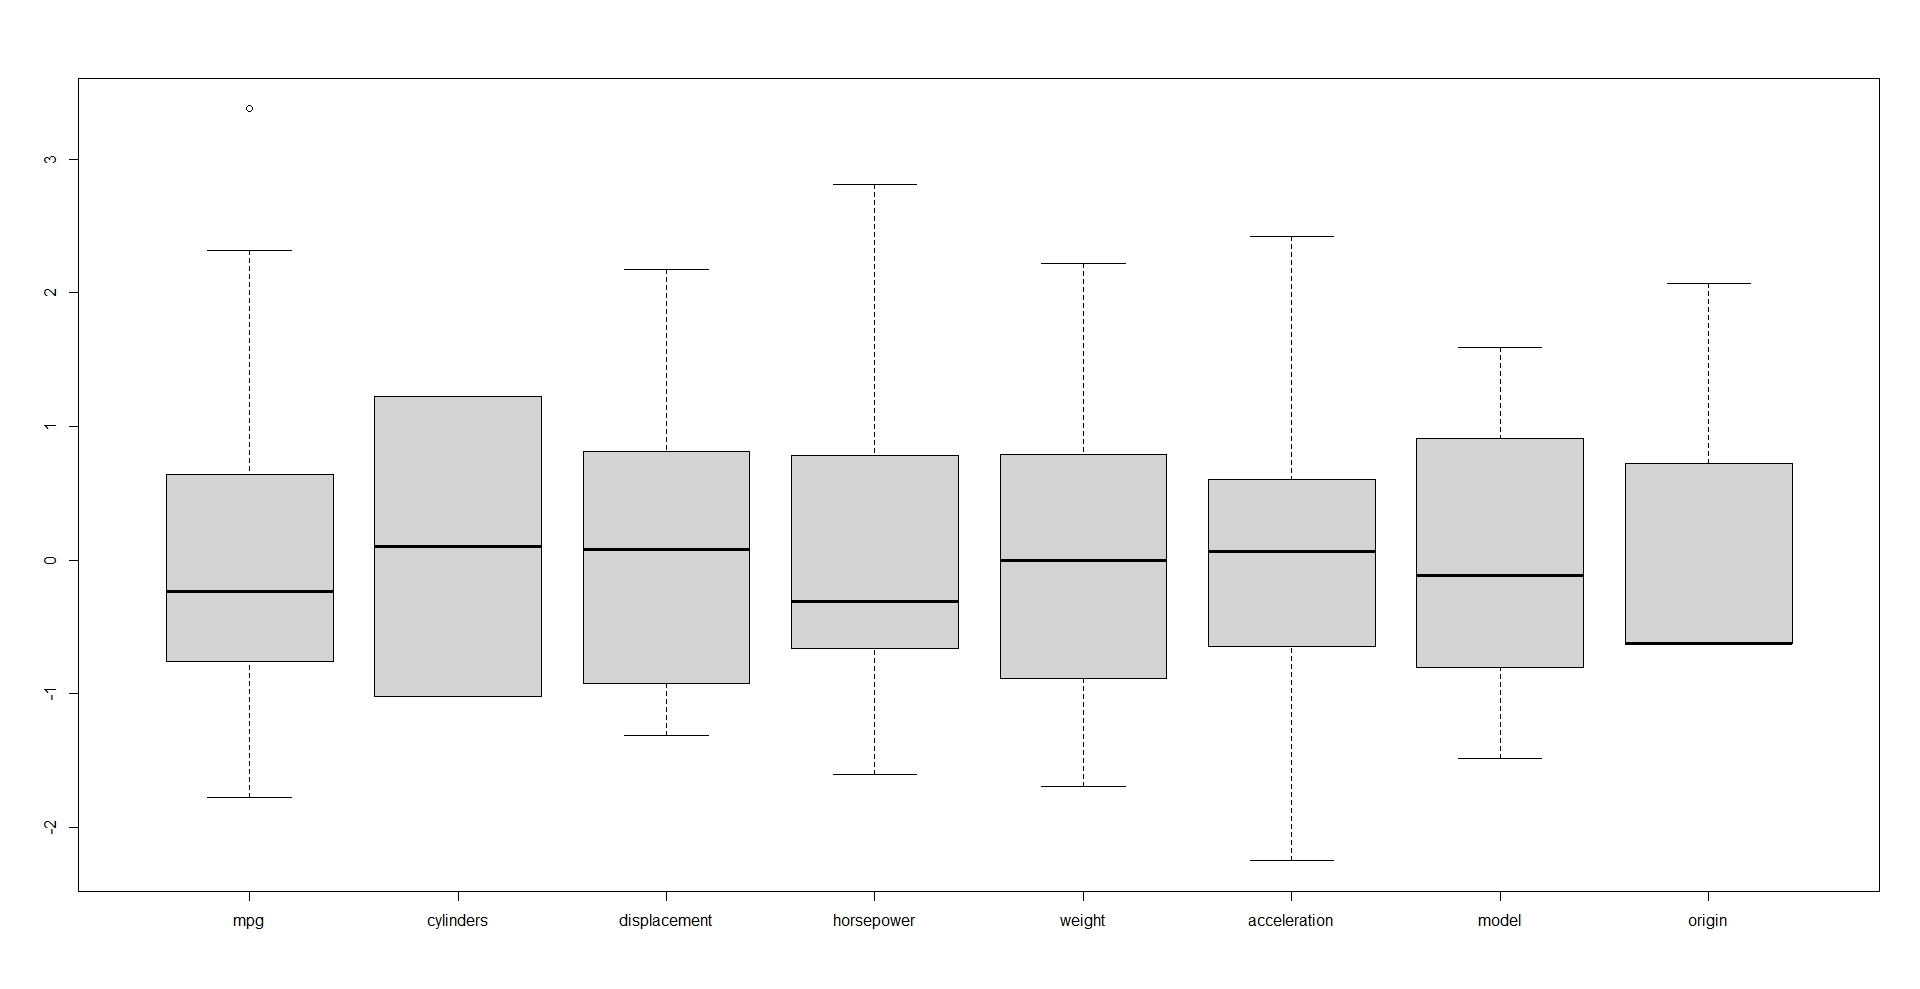
\includegraphics[width=\textwidth]{../boxplots/boxplot_scale_fig.jpeg}
            \end{figure}

            \begin{figure}[H]
                \caption{Histogram mpg}
                \centering
                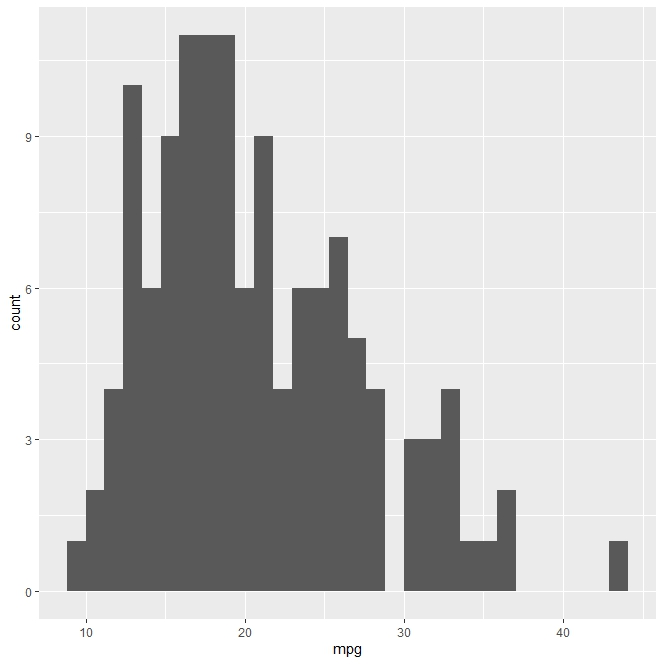
\includegraphics[width=0.7\textwidth]{../histograms/mpg_hist.jpeg}
            \end{figure}
            \begin{figure}[H]
                \caption{Histogram cylidnrów}
                \centering
                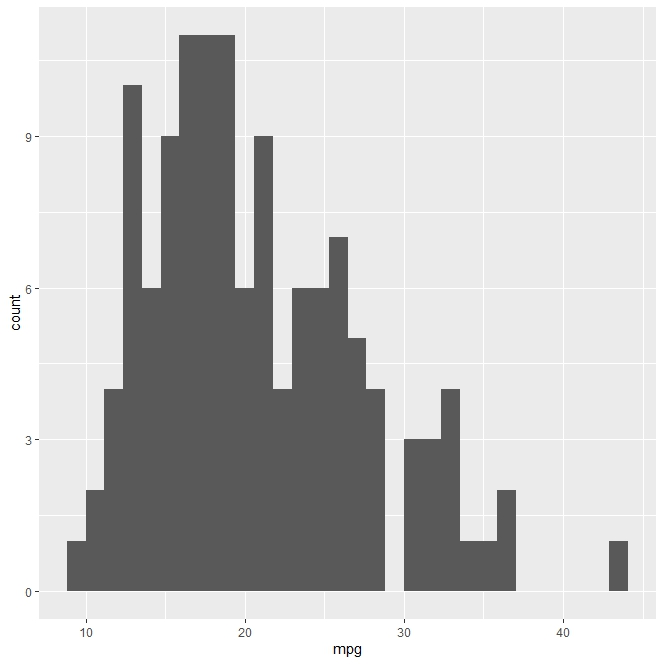
\includegraphics[width=0.7\textwidth]{../histograms/mpg_hist.jpeg}
            \end{figure}
            \begin{figure}[H]
                \caption{Histogram objętości skokowej silnika}
                \centering
                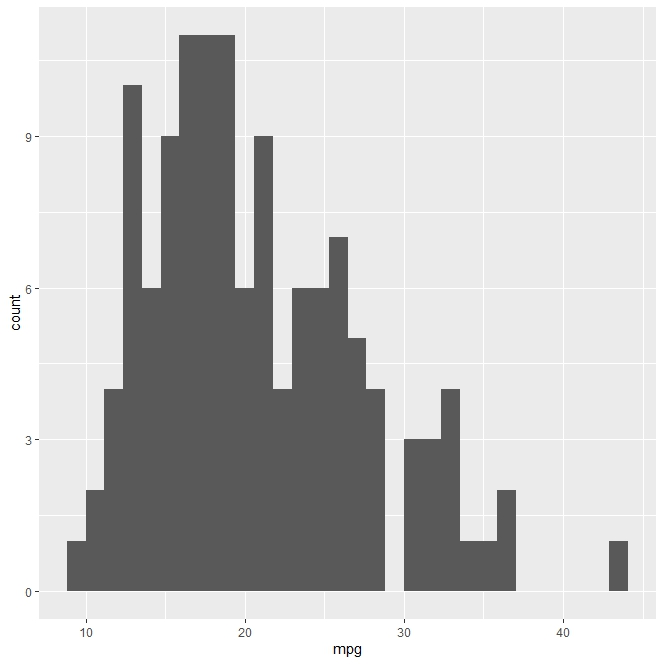
\includegraphics[width=0.7\textwidth]{../histograms/mpg_hist.jpeg}
            \end{figure}
            \begin{figure}[H]
                \caption{Histogram hp}
                \centering
                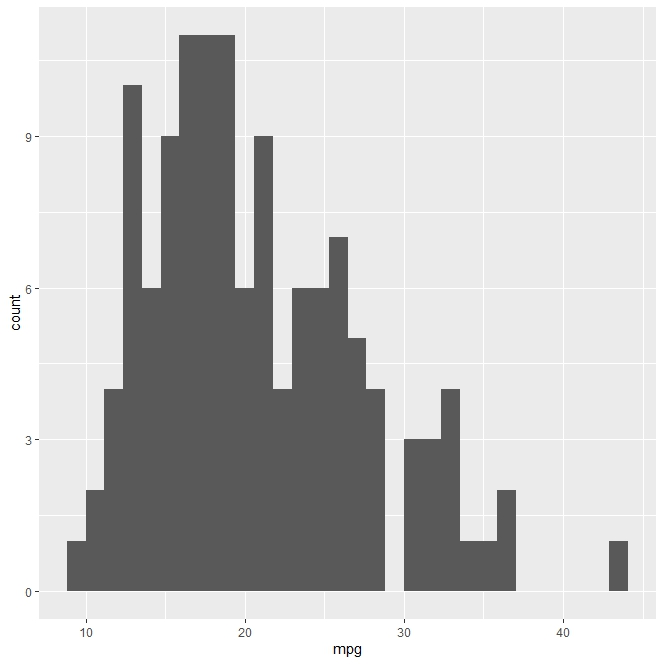
\includegraphics[width=0.7\textwidth]{../histograms/mpg_hist.jpeg}
            \end{figure}
            \begin{figure}[H]
                \caption{Histogram wagi}
                \centering
                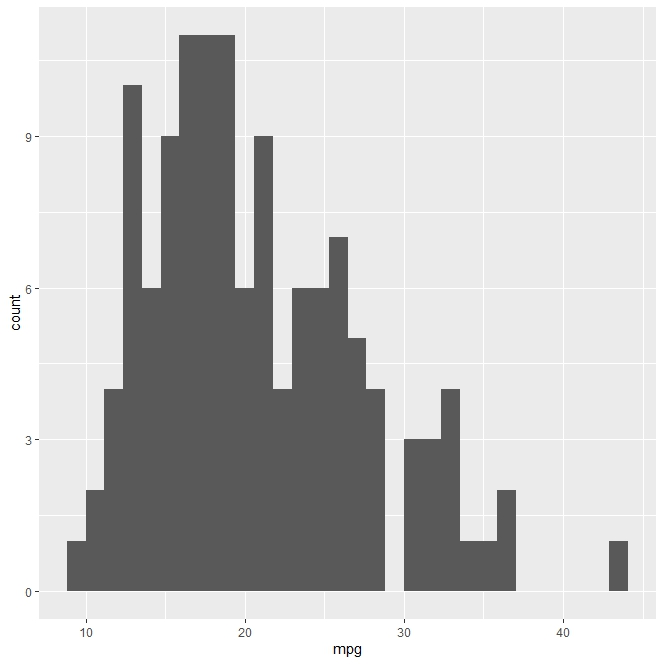
\includegraphics[width=0.7\textwidth]{../histograms/mpg_hist.jpeg}
            \end{figure}
            \begin{figure}[H]
                \caption{Histogram przyspieszenia}
                \centering
                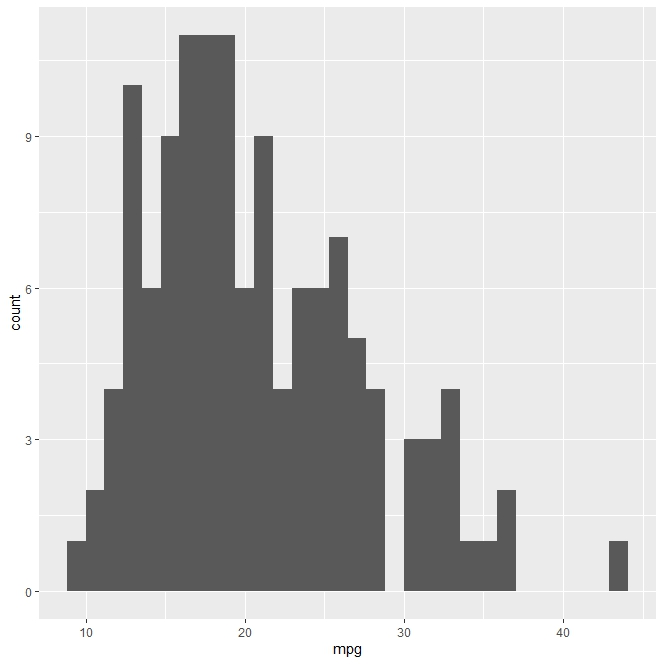
\includegraphics[width=0.7\textwidth]{../histograms/mpg_hist.jpeg}
            \end{figure}
            \begin{figure}[H]
                \caption{Histogram modelu}
                \centering
                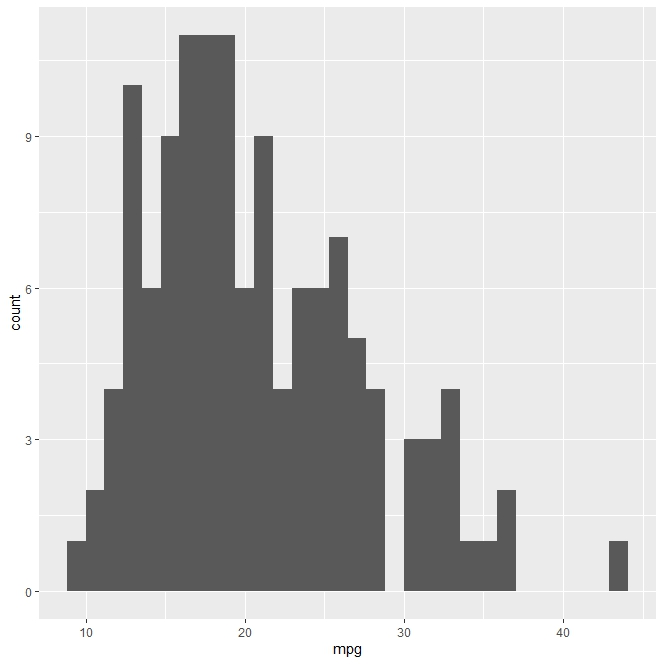
\includegraphics[width=0.7\textwidth]{../histograms/mpg_hist.jpeg}
            \end{figure}
            \begin{figure}[H]
                \caption{Histogram kraju pochodzenia}
                \centering0.7
                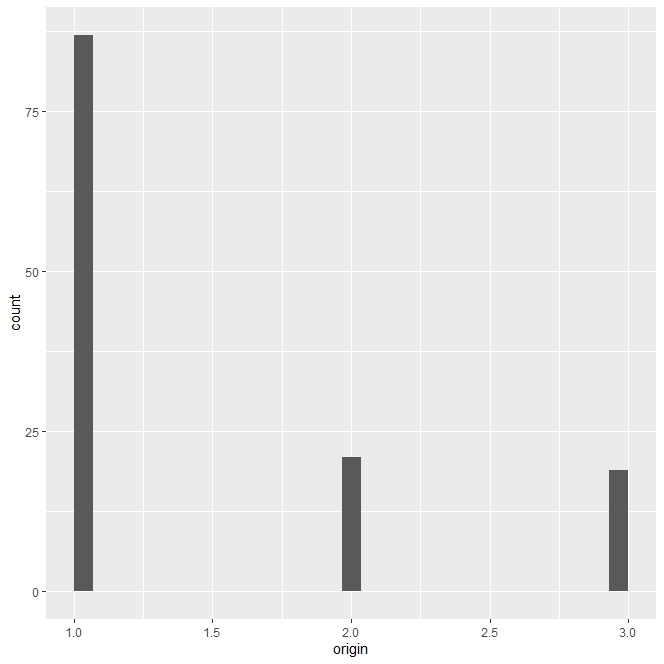
\includegraphics[width=0.7\textwidth]{../histograms/origin_hist.jpeg}
            \end{figure}
            
            
            
        \subsubsection*{Braki danych i ich obsługa}
        Braki danych występują jedynie dla cechy hp. Wszystkie samochody z brakiem danych zostały usunięte z danych za pomocą skryptu w R.
        \subsubsection*{Obserwacje odstające i ich obsługa}
            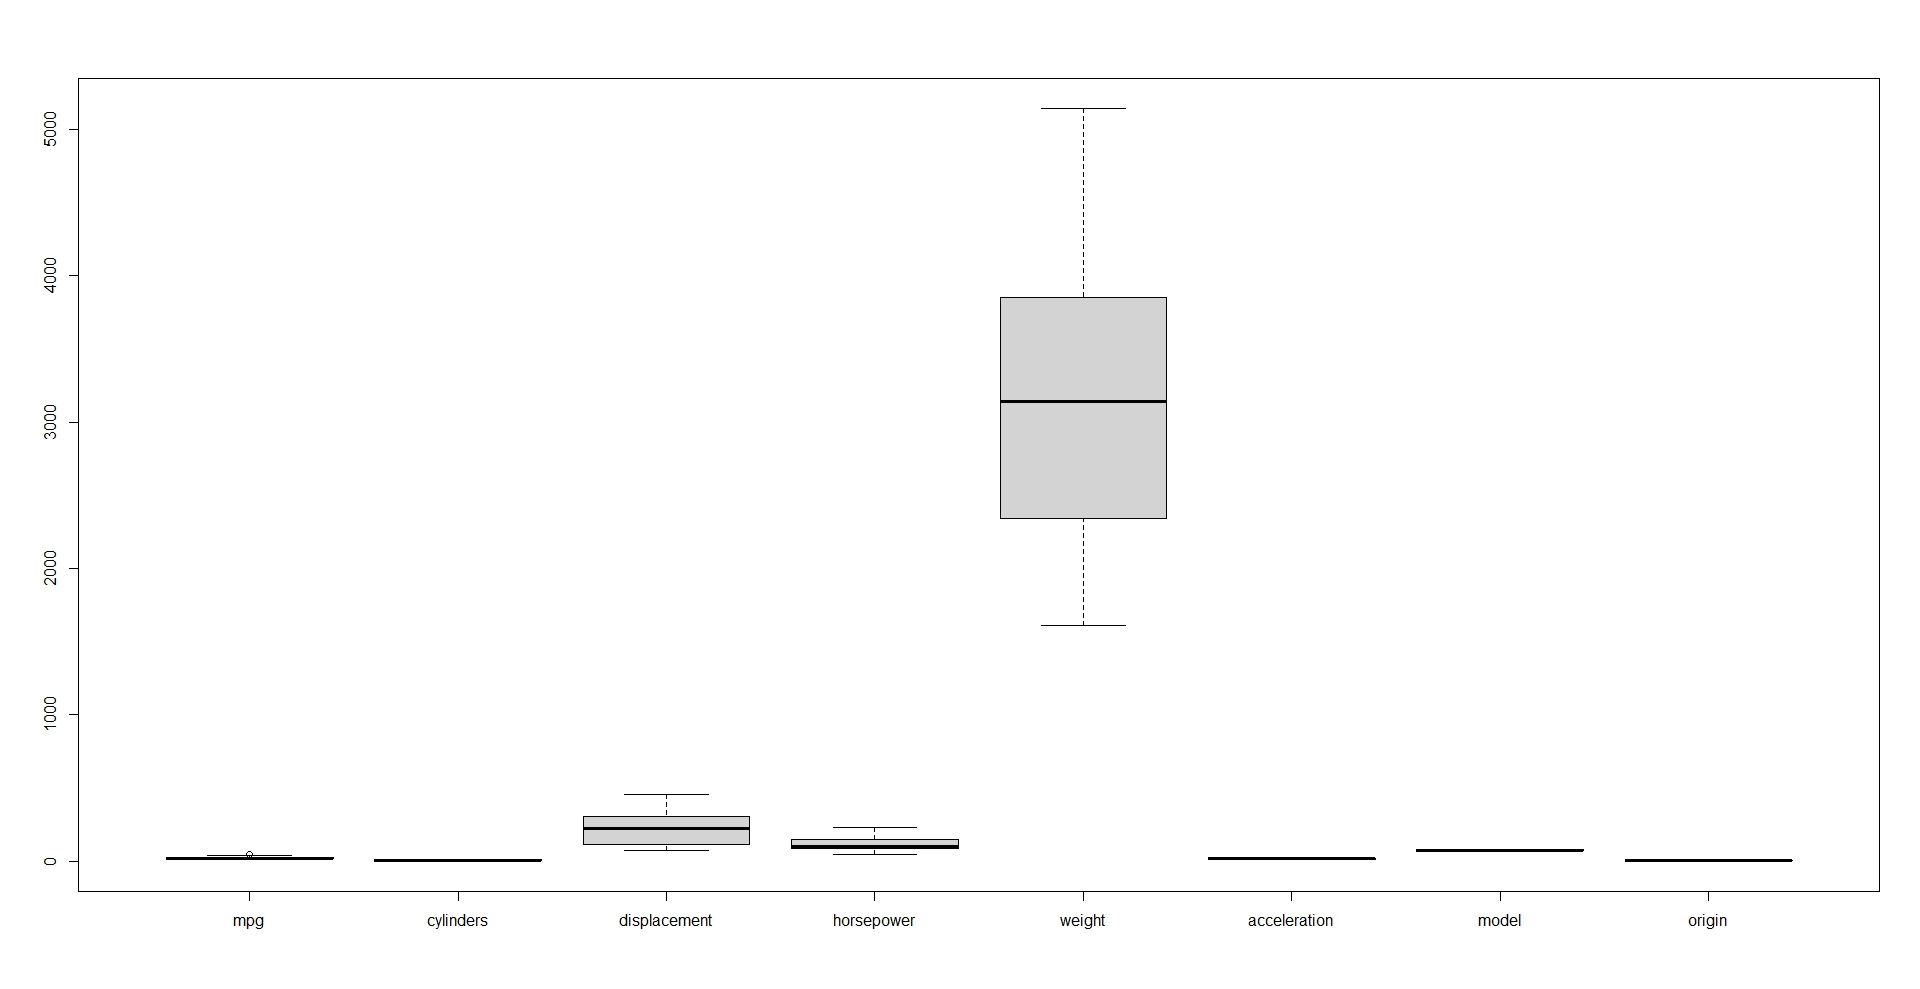
\includegraphics[width=\textwidth]{../boxplots/boxplot_noscale_fig.jpeg}
            Obserwacja odstająca występuje jedynie dla cechy mpg. Różnica wartości jest na tyle mała,
            że praktycznie nie wpływa na przebieg badania.
            

\section{Opis metod}
    \subsection{wzory wraz z opisami oznaczeń}
        \subsubsection*{Metoda k-średnich}
        Celem metody jest przypisanie do wektorów $r_i$ n wymiarowych wektorów danych,
        przy jak najmniejszym średnim błędzie kwantyzacji.
        Średni błąd kwantyzacji opisany jest wzorem:
            \begin{equation*}
                D = \frac{1}{K}\sum_{i=1}^{K} d(x_i, r)
            \end{equation*}
            \begin{itemize}
                \item K - liczba elementów ${x_i}$ przypisanych do wektora r
                \item d - miara błędu kwantyzacji, najczęściej błąd kwadratowy opisany wzorem:
                \begin{equation*}
                    d(x,r) = \sum_{j=1}^{n} (x_j - r_j)^2
                \end{equation*}
            \end{itemize}
        \subsubsection*{Metoda Warda}
            Odległość nowego skupienia od każdego pozostałego: 
            \begin{equation*}
                D_{pr} = a_{1}\cdot d_{pr} + a_{2}\cdot d_{qr} + b\cdot d_{pq}
            \end{equation*}
            \begin{itemize}
                \item r - numery skupień różne od p i q
                \item $D_{pr}$ - odległość nowego od skupienia r
                \item $d_{pr}$ - odległość pierwotnego skupienia p od skupienia r
                \item $d_{qr}$ - odległość pierwotnego skupienia q od skupienia r
                \item $d_{pq}$ - wzajemna odległość pierwotnych skupień p i q
                \item $a_{1} = \frac{n_{p} + n_{r}}{n_{p} + n_{q} + n_{r}}$, $a_{2} = \frac{n_{q} + n_{r}}{n_{p} + n_{q} + n_{r}}$, $b = \frac{-n_{r}}{n_{p} + n_{q} + n_{r}}$
                \item n - liczebność pojedyńczych obiektów w poszczególnych obiektach
            \end{itemize}
        \subsubsection*{SOM}
        Wzór aktualizowania neuronu v z wagą wektora $W_v(s)$:
            \begin{equation*}
                W_v(s+1) = W_v(s) + \theta(u,v,s) \cdot \alpha(s) \cdot (D(t)-W_v(s))
            \end{equation*}
            \begin{itemize}
                \item s - obecna iteracja
                \item t - indeks docelowego wektora danych wejściowych w zbiorze danych wejściowych D 
                \item D(t) - docelowy wektor danych wejściowych
                \item v - indeks wektora w mapie
                \item $W_v$ - aktualny wektor wagi węzła v
                \item u - to indeks BMU na mapie
                \item ${\theta(u,v,s)}$ - jest ograniczeniem ze względu na odległość od BMU, zwykle nazywaną funkcją sąsiedztwa
            \end{itemize}
    \subsection{cytowanie pracy w której zaproponowano metodę/ewentualnie pracy, w której użyto metodę} 
        \begin{quotation}
            \textit{"Metoda Warda dąży do uzyskania raczej małych skupień i jest uznawana za bardzo efektywną. W wyniku analizy otrzymujemy dendrogram,
            będący graficzną interpretacją uzyskanych efektów. W zależności od przyjętych założeń badania, w tym zwłaszcza akceptowanej odległości
            taksonomicznej między obiektami ze względu na zaproponowany zestaw cech, możemy wyróżniać większe lub mniejsze skupienia, a co za tym
            idzie – mniejszą lub większą ich liczbę."}
            - Grupowanie państw Unii Europejskiej ze względu na zasoby kapitału ludzkiego i intelektualnego - Dr Małgorzata Stec, 
            Mgr Agata Janas, Mgr Artur Kuliński - Uniwersytet Rzeszowski
        \end{quotation}
        \begin{quotation}
            \textit{"Dla potrzeb klasyfikacji bezwzorcowej skonstruowano sieć typu SOM. Jest to jeden z najbardziej zaawansowanych 
            modeli sieci neuronowych, który dostarcza topologicznego odwzorowania przestrzeni wielowymiarowej na dwuwymiarową mapę neuronów. 
            Może ona być zastosowana do wizualizacji skupisk w zbiorze danych, zachowując nieliniowe relacje między jednostkami i lokując 
            bliskie jednostki bliżej siebie. Podczas trenowania sieci SOM wagi neuronów modelowane są w taki sposób, by bardzo zbliżone do 
            siebie przypadki reprezentował ten sam neuron, a podobne reprezentowane były przez neurony sąsiednie."}
            - Grupowanie państw Unii Europejskiej ze względu na zasoby kapitału ludzkiego i intelektualnego - Dr Małgorzata Stec, 
            Mgr Agata Janas, Mgr Artur Kuliński - Uniwersytet Rzeszowski
        \end{quotation}
    

\section{Rezultaty w postaci graficznej oraz omówienie wyników}
    \subsection{Metody wyznaczania optymalnej liczby zbiorów}
        \subsubsection{Metoda łokciowa}
            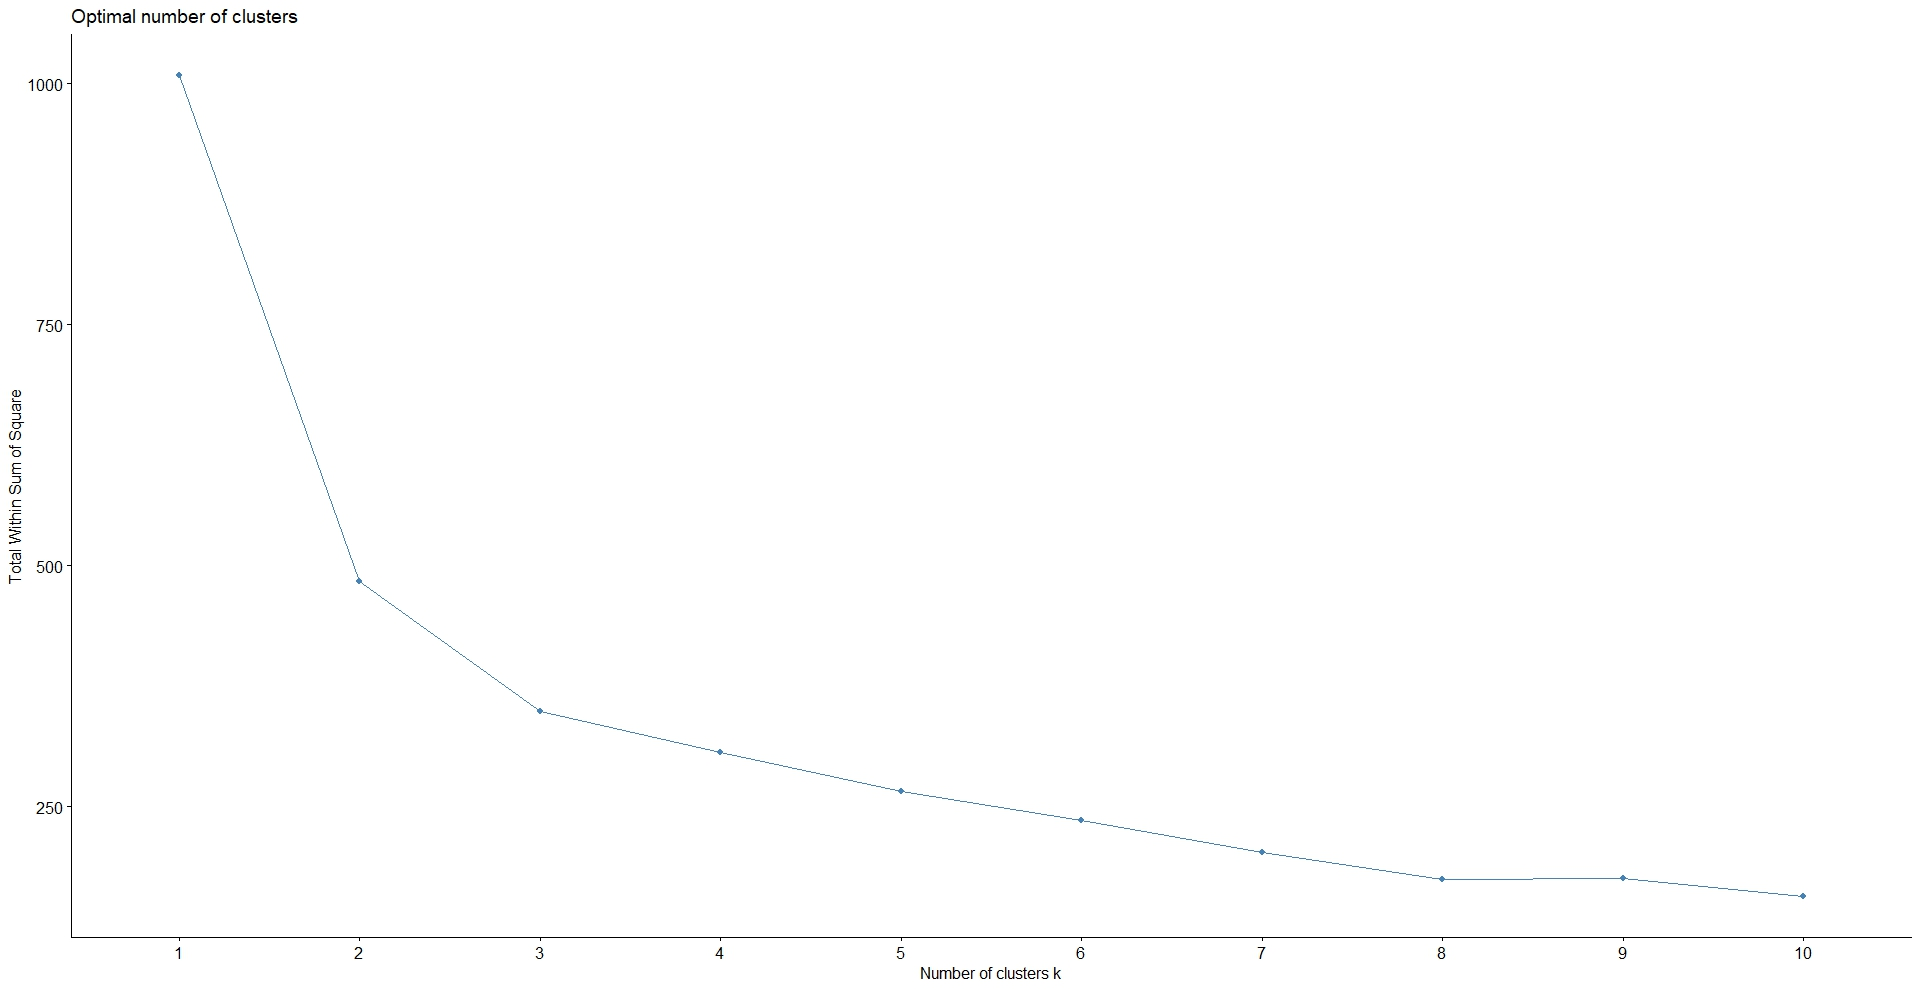
\includegraphics[width=\textwidth]{elbow_fig.jpeg}
            Z wykresu metody łokciowej można zaobserwować, że od wartości 3 na osi poziomej 
            wykres maleje liniowo, więc ten punkt możemy przyjąć jako liczbę zbiorów do 
            naszych danych.
        \subsubsection{Metoda silhouette}
            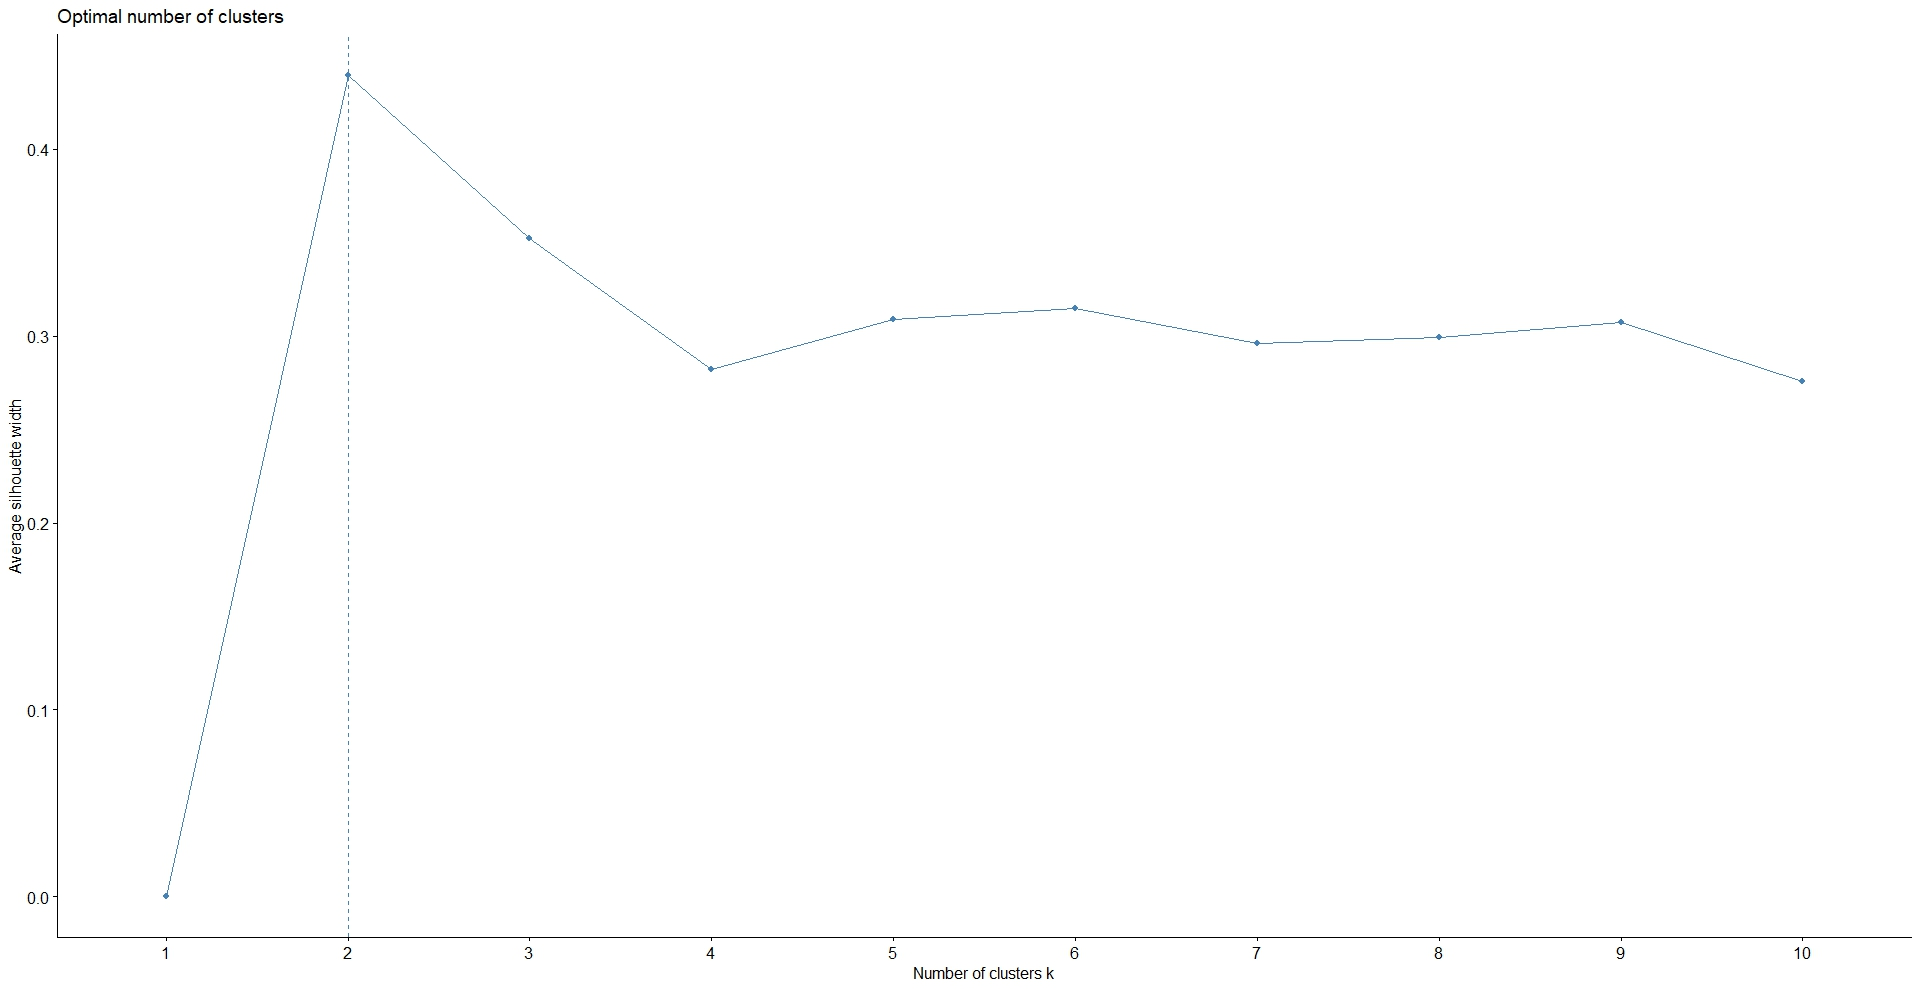
\includegraphics[width=\textwidth]{silhouette_fig.jpeg}
            Kolejna metoda to ustalenia odpowiedniej liczby grupy, skupisk do naszych danych. 
            Z tej metody wyszło, że nasze dane powinny być podzielone na 2 grupy. Ostatecznie 
            wybraliśmy wybraliśmy 3 grupy zgodnie z metodą łokciową.
    
    \subsection{Metoda k-średnich}    
        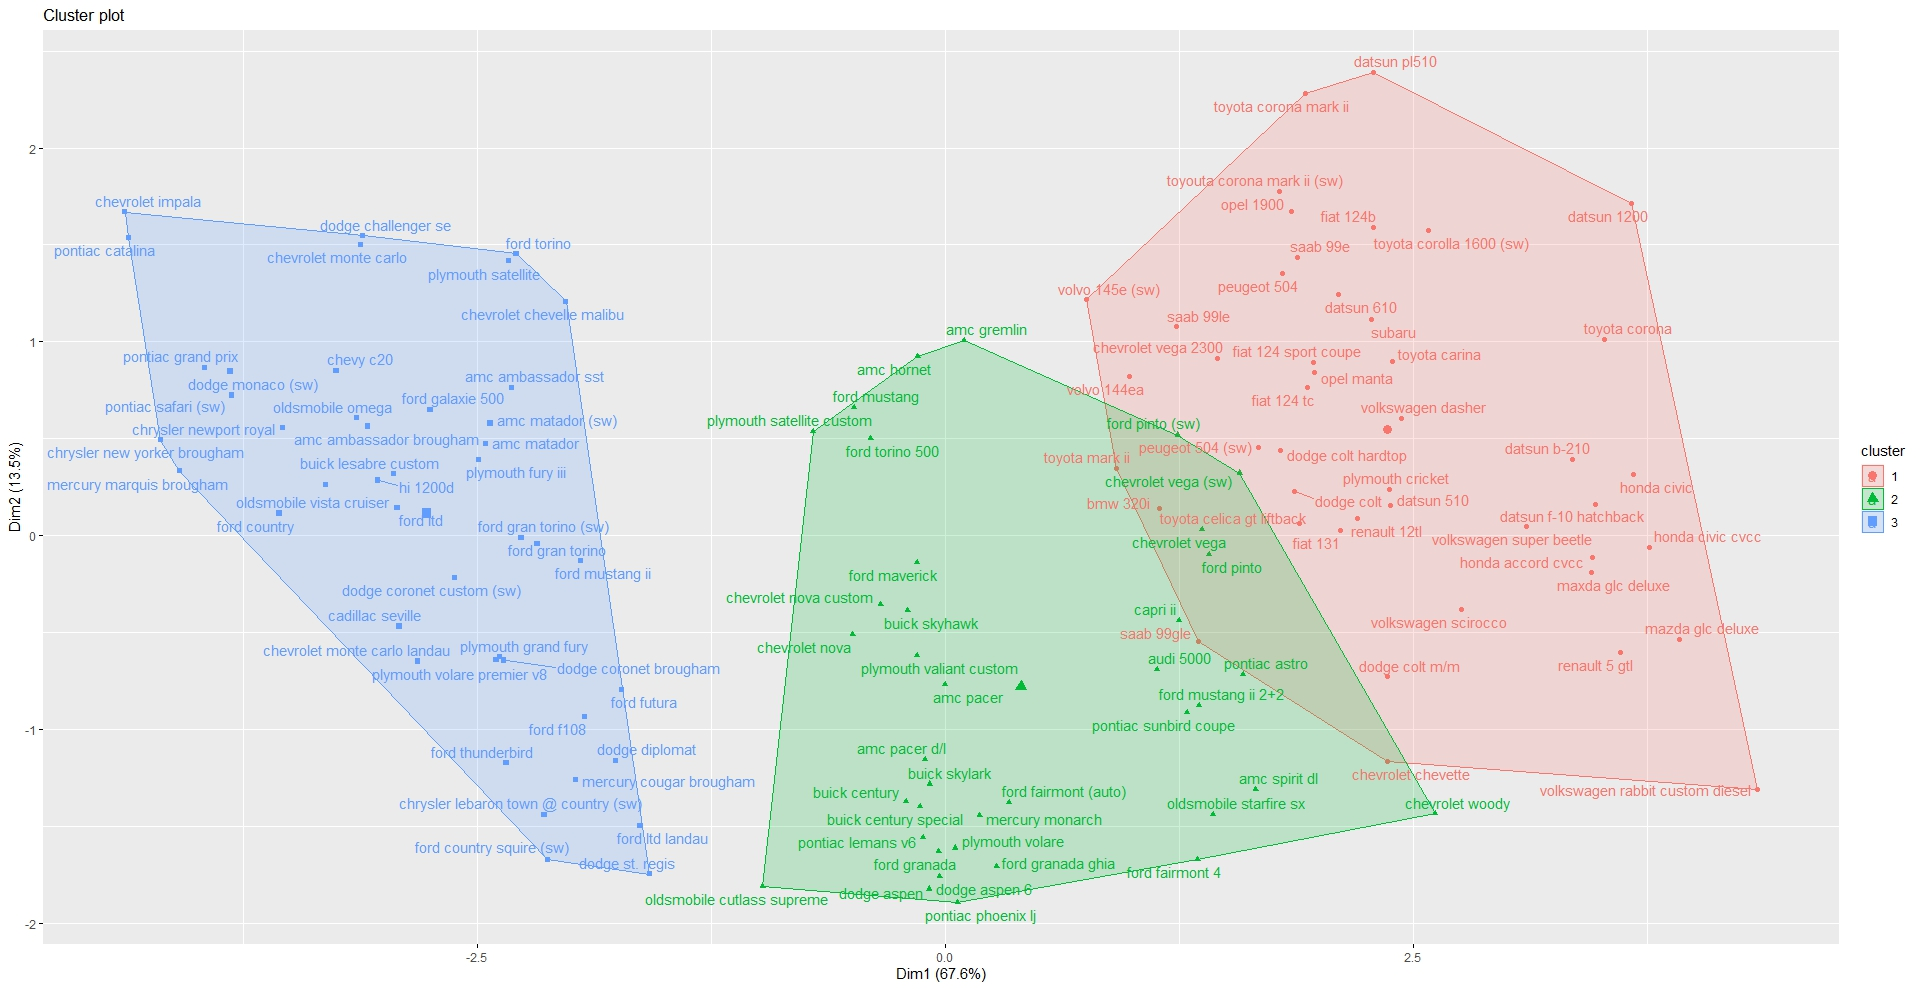
\includegraphics[width = \textwidth]{kmeans_fig}
        Dzięki metodom, które pomagają wybrać optymalną liczbę grup mogliśmy przeprowadzić analizę metodą k-średnich. 
        Nasza optymalna liczba grup to 3. Z tego wykresu możemy odczytać zbiory o podobnych elementach oraz odległość między nimi. 
        Co świadczy o wielkości podobieństwa. Na naszym wykresie można dostrzec, że dwa zbiory się pokrywają co świadczy o tym, że dane, 
        które znajdują się w obu zbiorach kwalifikują się zarówno do zbioru zielonego i czerwonego, czyli ich parametry są do siebie zbliżone.
        \newline\newline
        W zbiorze niebieskim są tylko samochody pochodzenia amerykańskiego, a w zbiorach zielonym i czerwonym są samochody pochodzenia 
        europejskiego i japońskiego. Samochody amerykańskie charakteryzuje duża pojemność silnika, wysoka objętość skokowa silnika, duża 
        waga oraz niskie mpg.

        
    \subsection{Metoda Warda}
        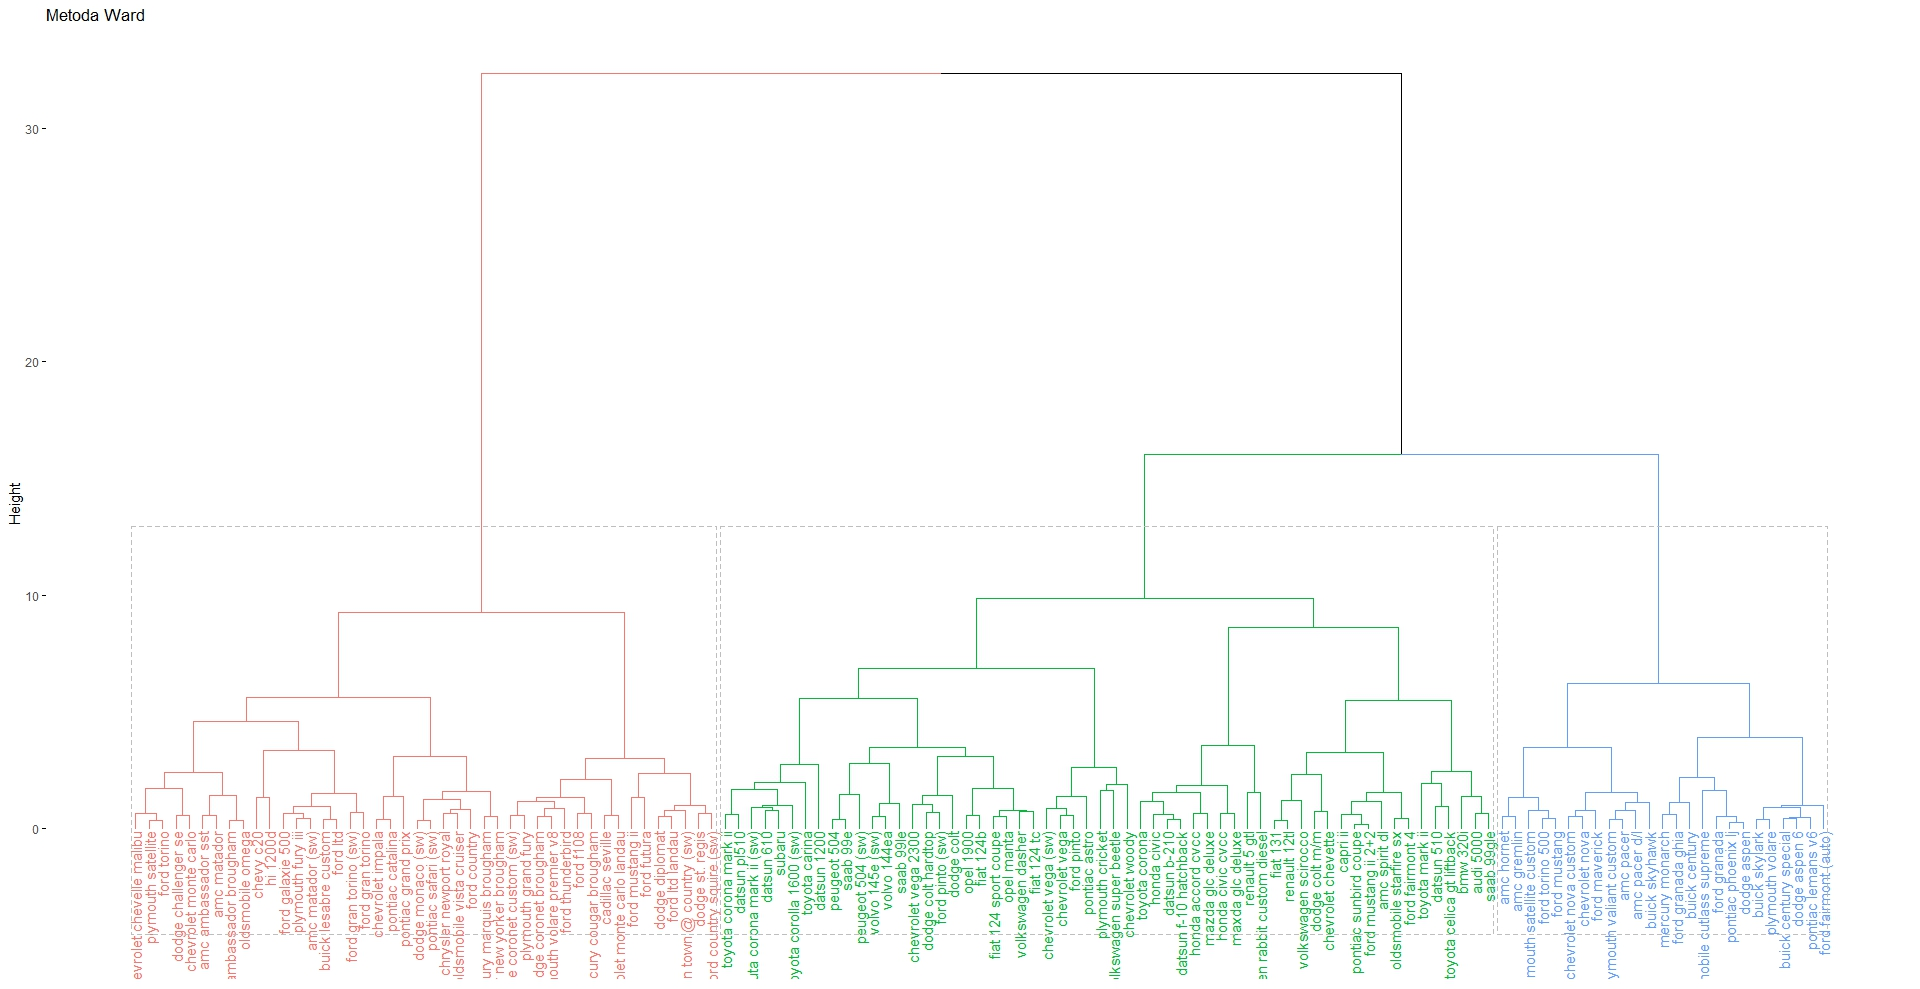
\includegraphics[width = \textwidth]{ward_fig}
        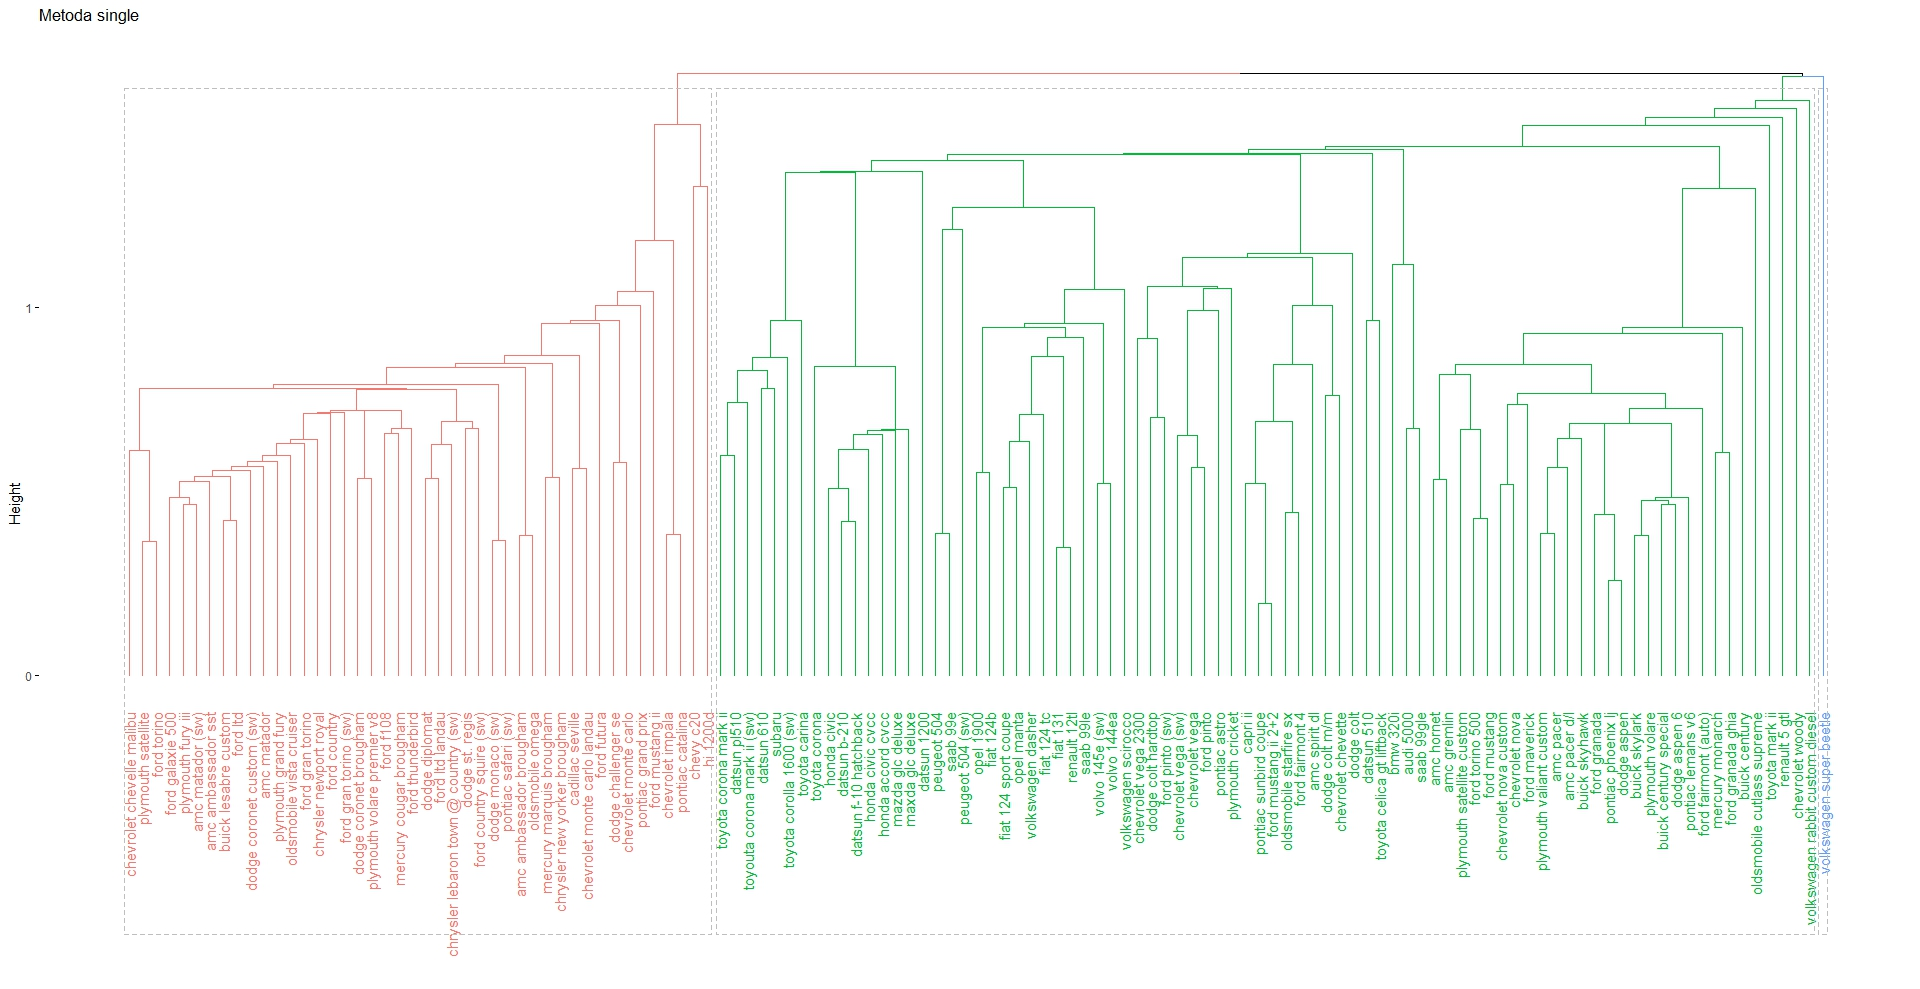
\includegraphics[width = \textwidth]{single_fig.jpeg}
        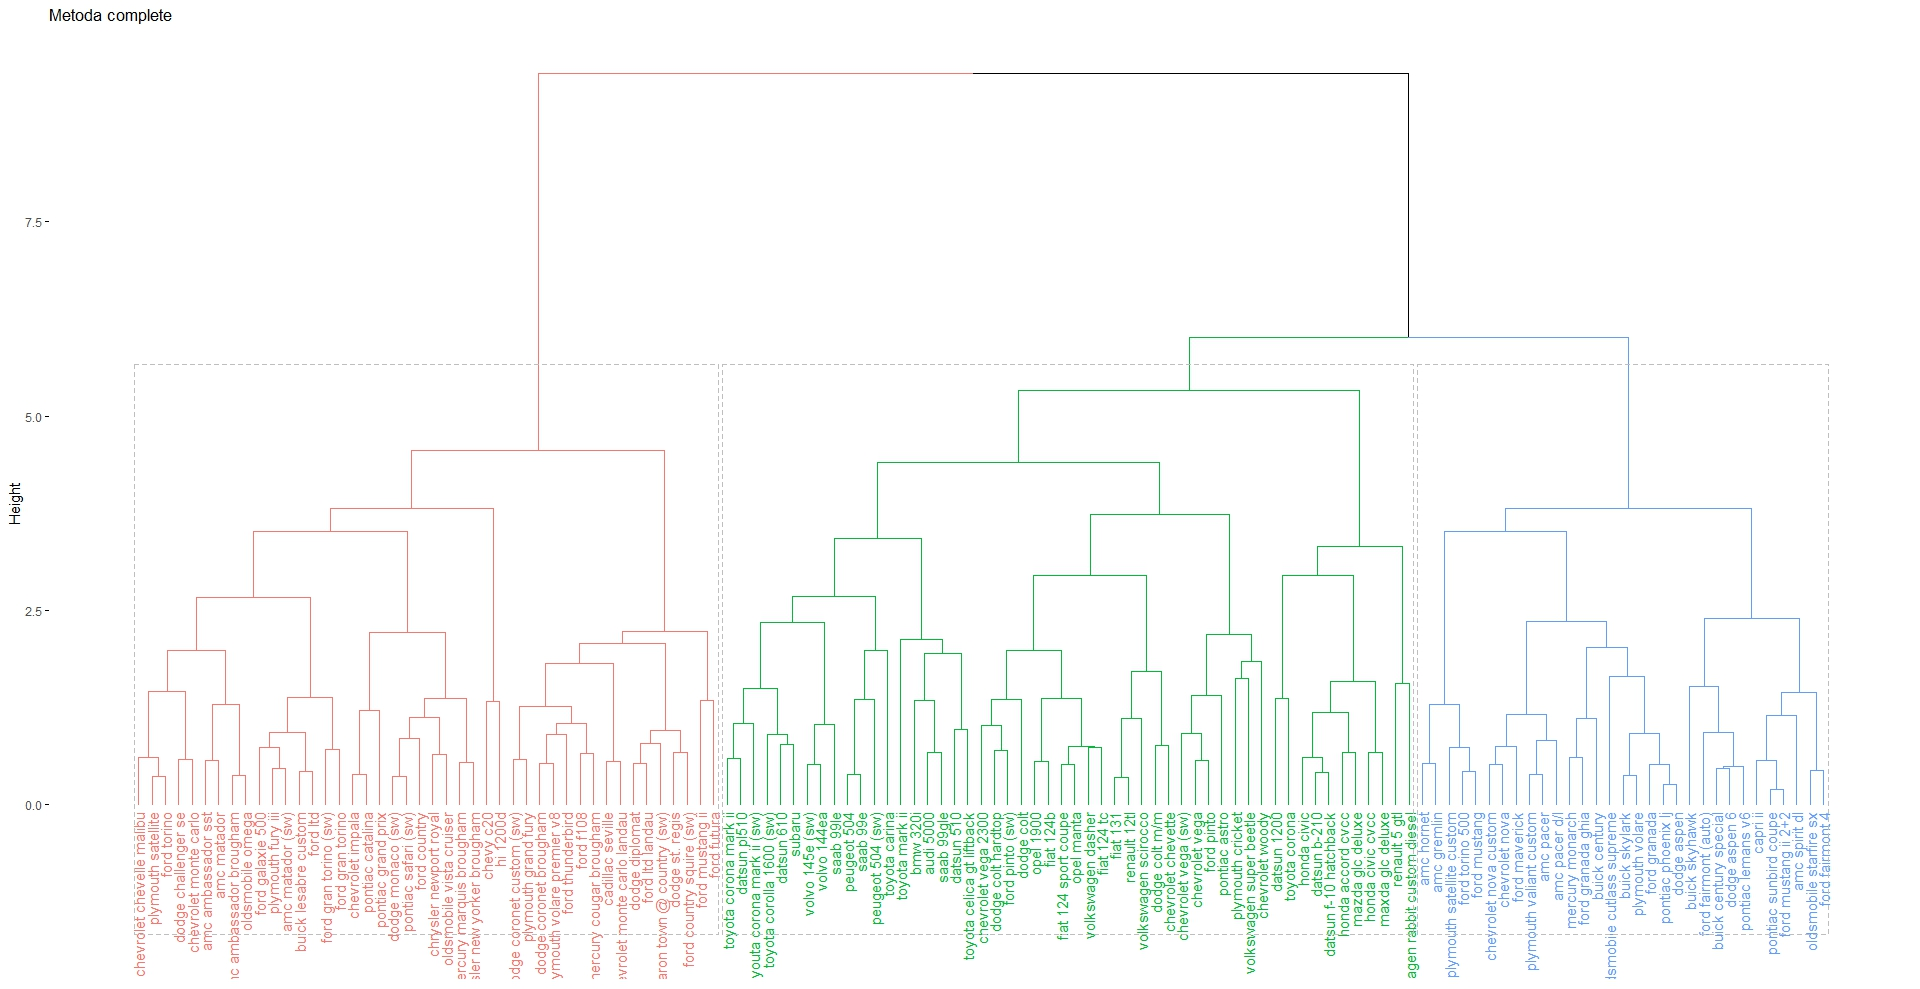
\includegraphics[width = \textwidth]{complete_fig.jpeg}
        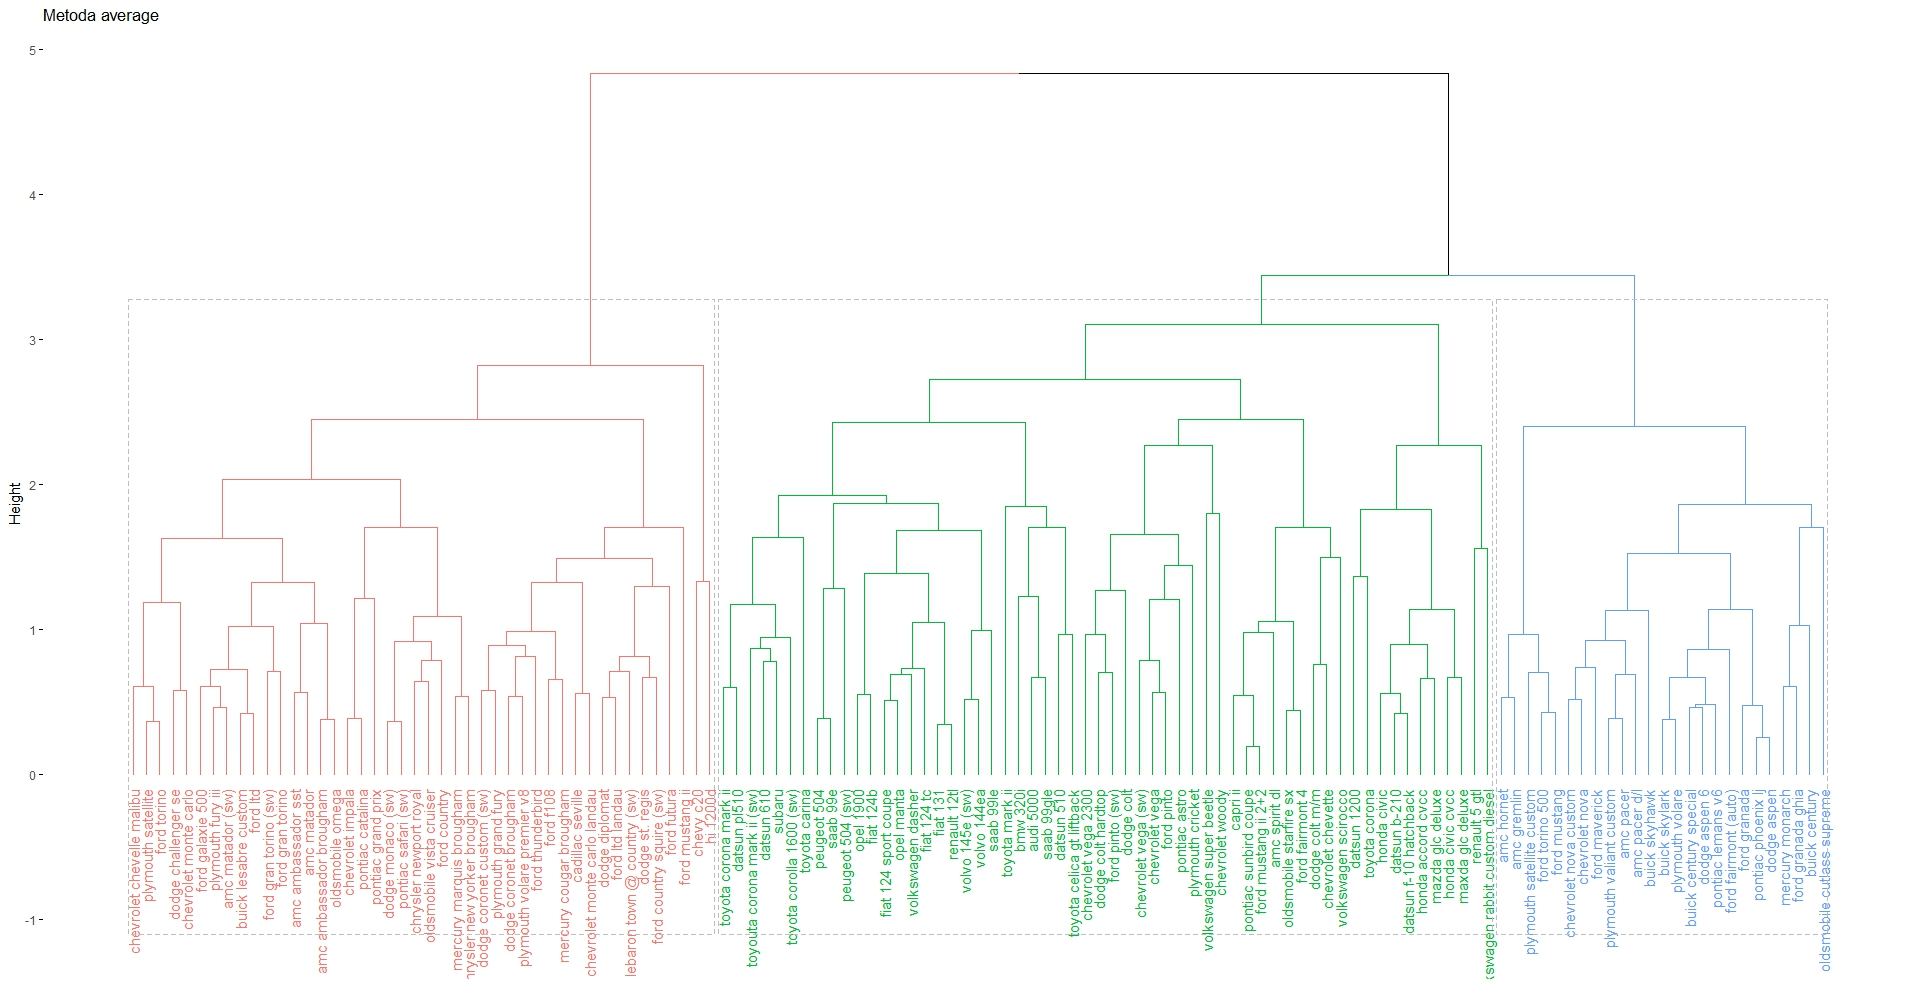
\includegraphics[width = \textwidth]{average_fig.jpeg}
        Jak widzimy wykresy wyglądają bardzo różnie. Grupy znalezione metodą Warda mają zbliżone wielkości. W przypadku metody single  wykres 
        jest najmniej czytelny oraz w klastrze trzecim, czyli niebieskim występuje tylko jeden obiekt. W tej metodzie grupa druga, czyli zielona 
        przyjęła elementy z grupy niebieskiej porównując do reszty metod łączenia. Metoda Warda ma najbardziej czytelny wykres, łatwo z niego 
        można odczytać otrzymane wyniki. Wykresy metod complete oraz average są dosyć podobne do siebie. 
        Można zauważyć również, że zbiory zielone i niebieski się zawsze łączą a dopiero później łączą się z ostatnim czerwonym. Wynika z tego 
        więc, że zbiór zielony i niebieski mają więcej wspólnych cech niż z zbiorem czerwonym. W przypadku wykresu complete wysokość osiąga 
        wartość 8, w average około 5, w single około 1.5 i w metodzie Warda około 33. Im większa wysokość tym mniejsze powiązanie między 
        aglomeracjami. Z tego wynika, że w metodzie single jest najmniejsza różnica powiązań, a w metodzie Warda najmniejsza.


    \subsection{SOM}
        \subsubsection{SOM counts}    
            Rozmiar siatki to $5\times4$
            \newline
            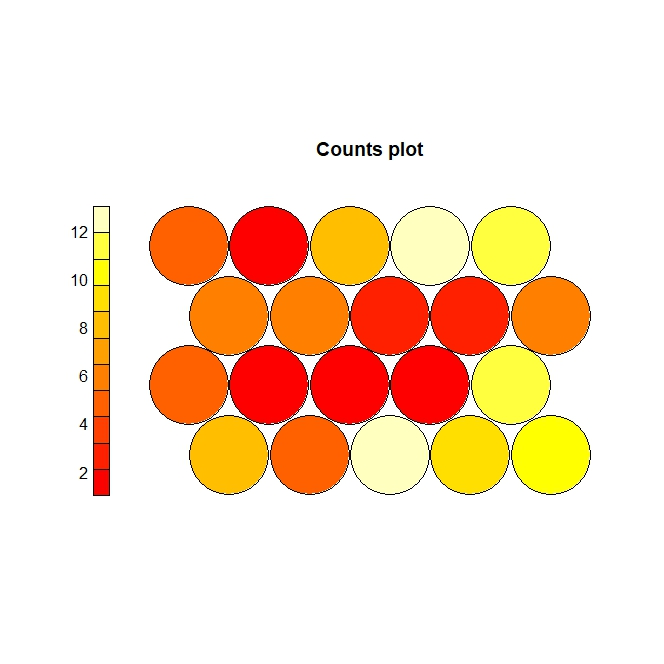
\includegraphics[width = \textwidth]{som_counts_fig.jpeg}
            Ustawiliśmy siatkę w wymiarach x = 5 i y = 4, ponieważ przy takich wymiarach nie pojawiają się 
            szare okręgi, czyli takie, które są puste. Przy takich wymiarach siatki liczebność zbiorów liczy od 1 do 14. 
            Największe zbioru są w prawym dolnym rogu, na środku przy dolnej krawędzi wykresu oraz w prawym górnym rogu. 
            Zbiory o najmniejszej liczbie elementów mieszczą się w środku. Po lewej stronie ziobry mają po około 6 elementów.

        \subsubsection{SOM codes}   
            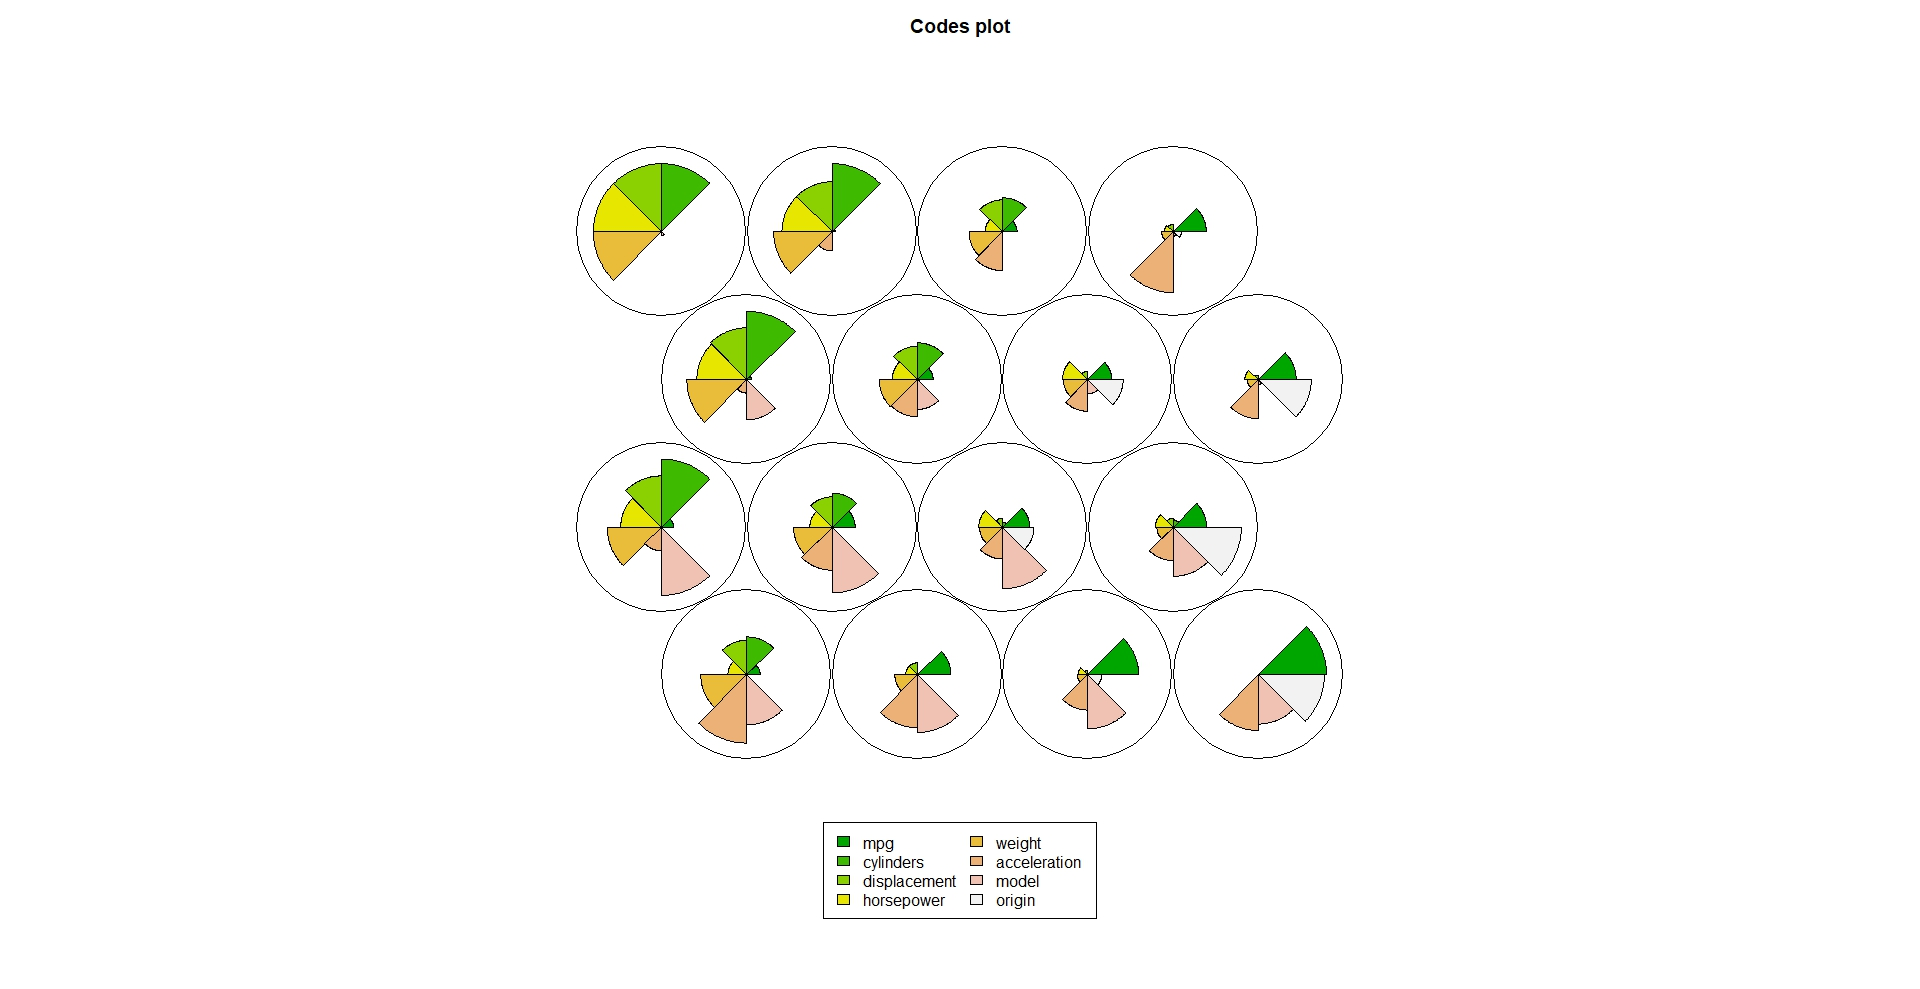
\includegraphics[width = \textwidth]{som_codes_fig.jpeg}
            W prawym dolnym rogu są zbiory według liczby cylindrów, objętości skokowej silnika, liczby koni mechanicznych i wagi. 
            Były to też najliczniejsze zbiory według wykresu som counts. Od środka do lewej strony widać, że zbiory są dobierane według 
            modelu, czyli roku produkcji. W środku duże znaczenie ma pochodzenie samochodu.

        \subsubsection{SOM neighbour distance}
            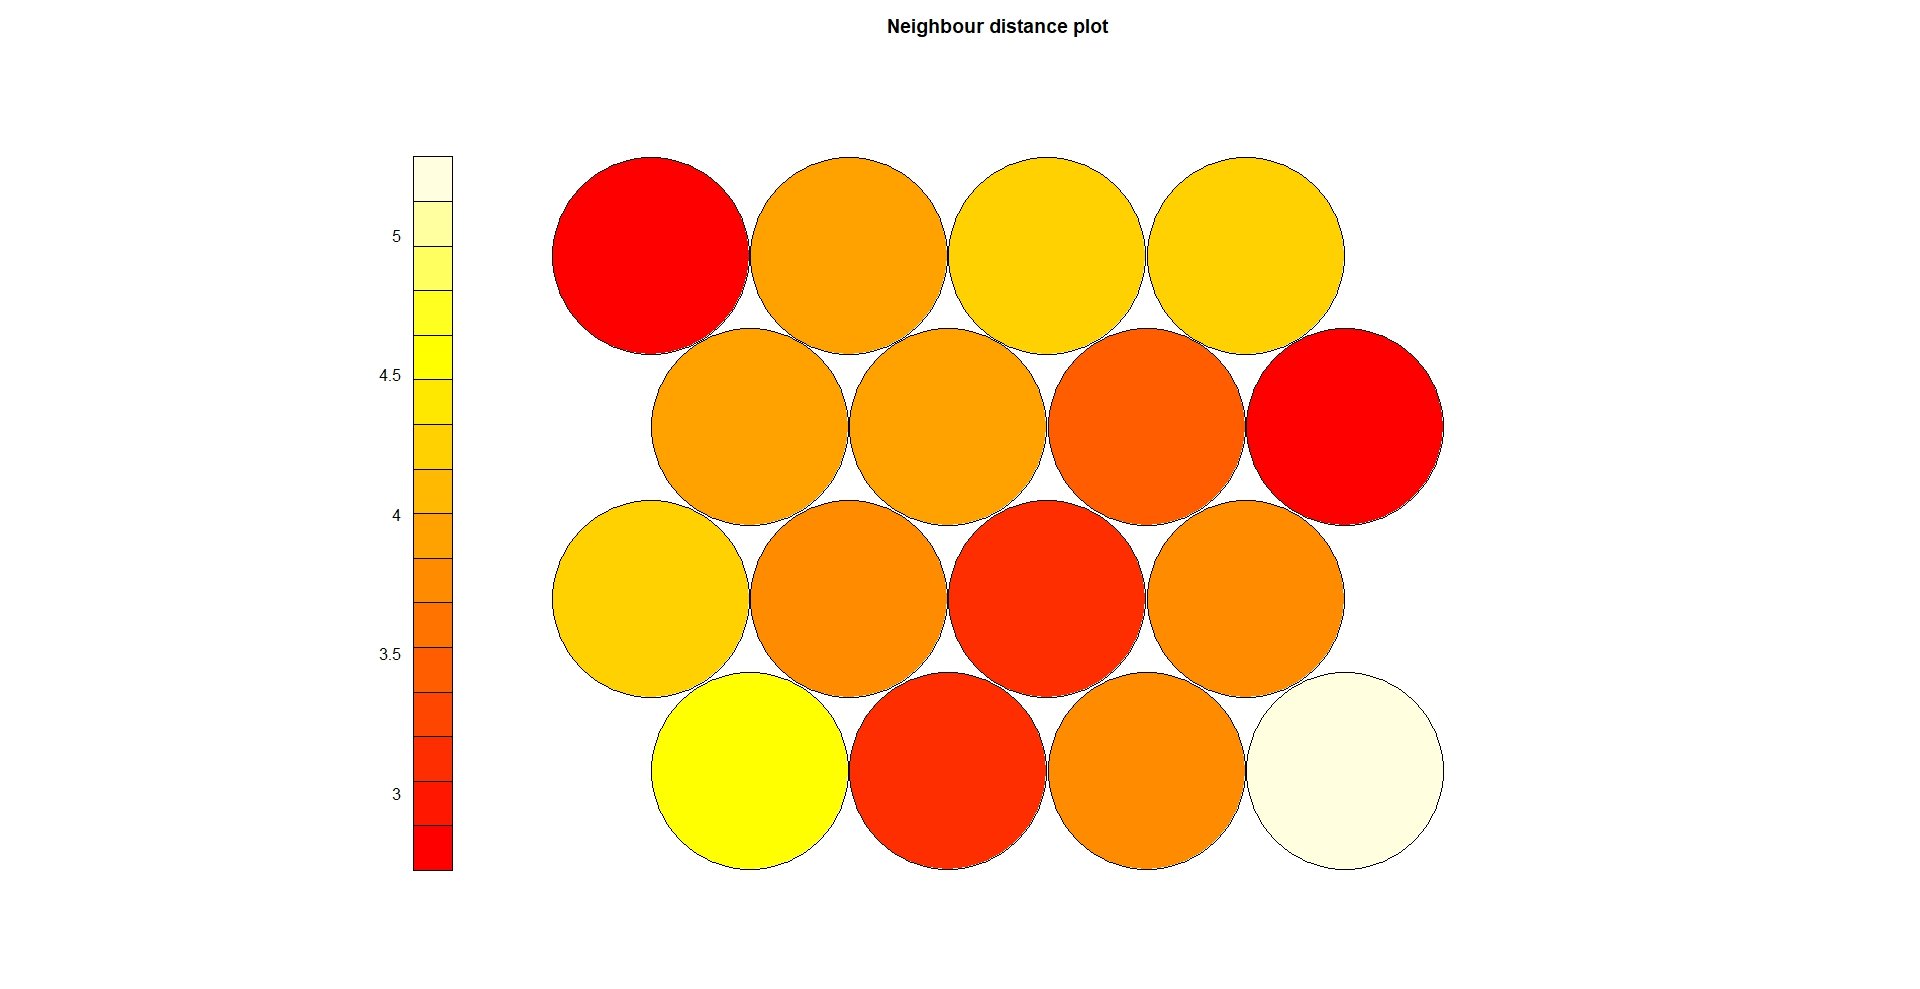
\includegraphics[width = \textwidth]{som_neighbour_dist_fig.jpeg}
            Skala od 0 do 6. Najmniejsze odległości między zbiorami można zaobserwować w lewym dolnym roku oraz w prawym dolnym rogu. 
            W drugim i trzecim wierszy od środka w prawo są największe odległości między zbiorami, co oznacza, że mają mniej wspólnych cech. 
            Reszta zbiorów ma odległość na poziomie około 4, według skali przedstawionej na wykresie. 

        \subsubsection{SOM training progress}
            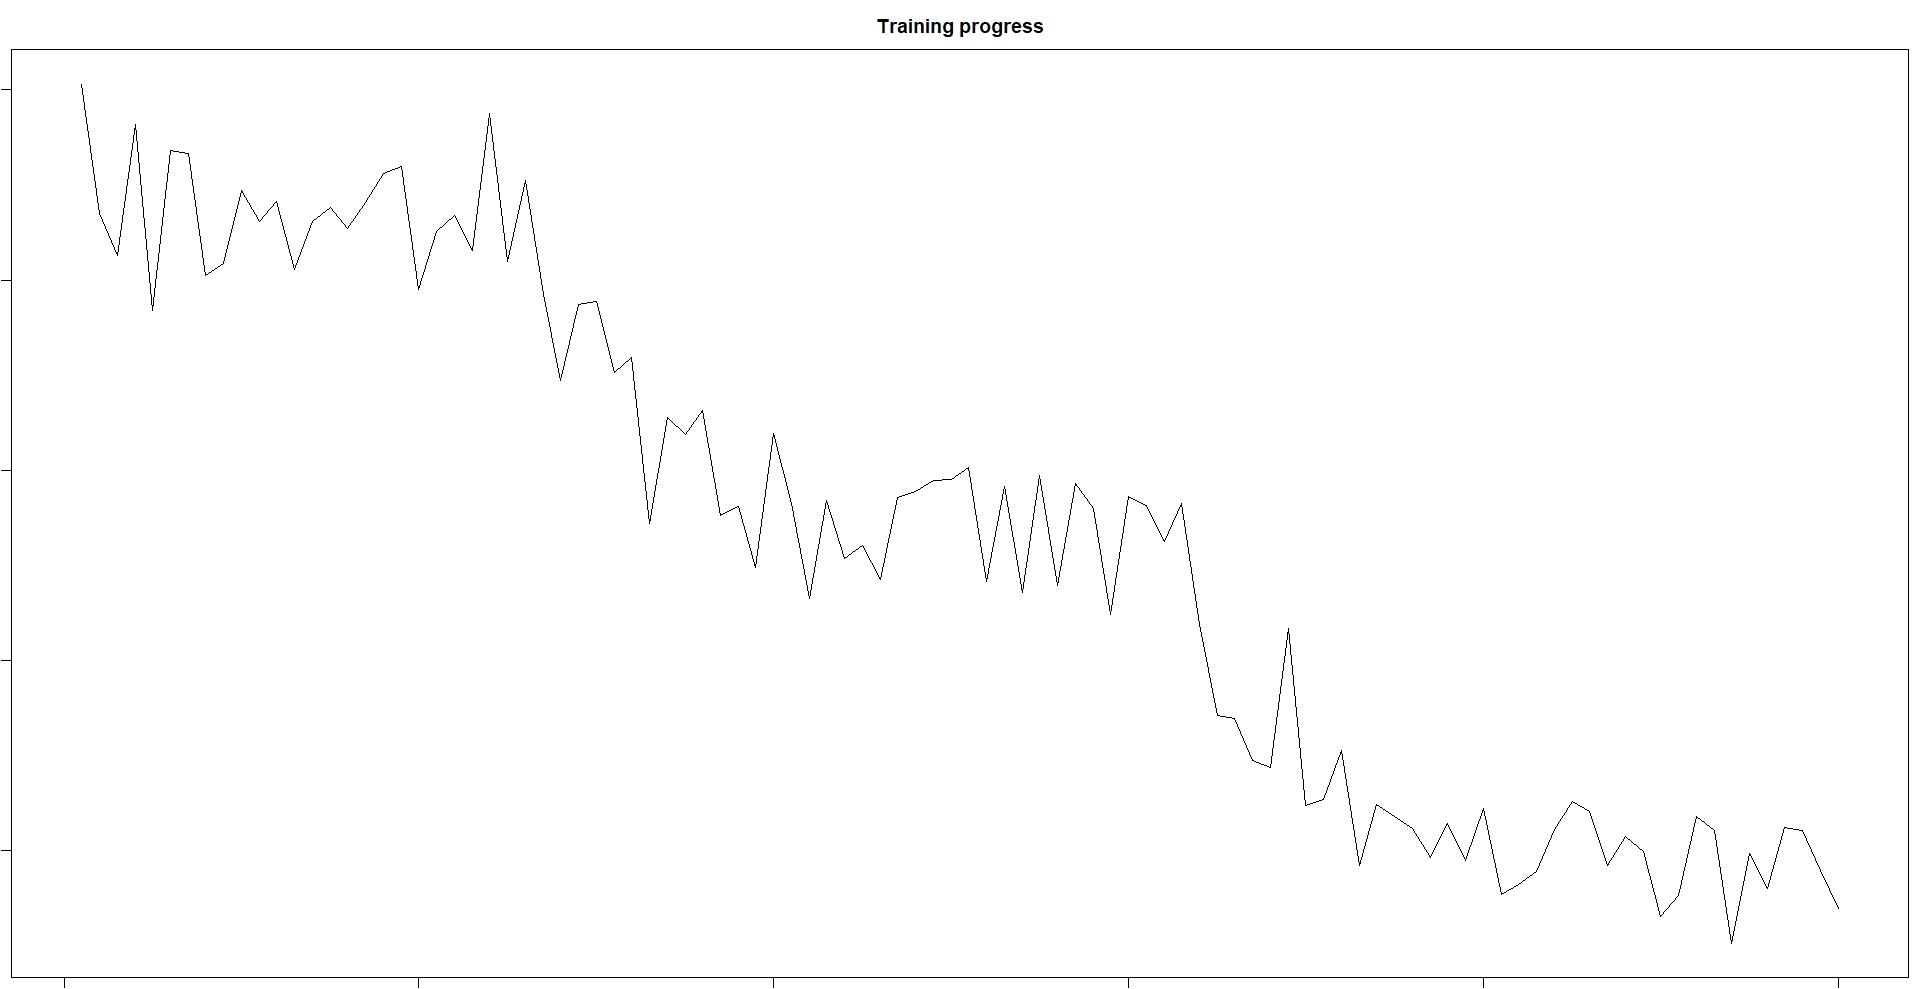
\includegraphics[width = \textwidth]{som_changes_fig.jpeg}
            Oś x to liczba iteracji a oś y to średnia odległość do najbliższej jednostki
            W miarę postępu iteracji uczenia SOM zmniejsza się odległość od wag każdego węzła do próbek reprezentowanych przez ten węzeł.
            Idealna odległość powinna osiągnąć minimalny poziom plateau. Ta opcja wykresu pokazuje postęp w czasie. Na naszym wykresie widać 
            jak pod koniec funkcja coraz wolniej maleje, ale nadal występuje duża fluktuacja danych. 
            Problem Plateau polega na wykazaniu istnienia minimalnej powierzchni przy danej granicy.

\section{Podsumowanie (ocena realizacji celu, odniesienie do pozycji z przeglądu literatury)}
Na podstawie przeprowadzonych szacowań optymalnej liczby skupisk metodą łokciową i silhouette wnioskujemy, że optymalnym wynikiem są 
trzy skupiska. Wykorzystaliśmy metodę k-średnich dla trzech centroidów oraz metodę Warda dla trzech klastrów. Wynikiem przeprowadzonych 
działań jest podział samochodów na trzy skupiska. Metoda Warda przestawia bardziej szczegółowo podobieństwo między poszczególnymi 
samochodami. Ponadto dzieli ona również wynik na trzy rozłączne względem siebie klastry, a w metodie k-średnich występują elementy należące 
do dwóch klastrów. W obu metodach klaster niebieski składa się wyłącznie z samochodów pochodzenia amerykańskiego. 
Można to uznać za sukces, ponieważ samochody tego pochodzenia, szczególnie w latach 1970-82 tworzyły unikalny segment 
rynku oparty o wysoką wydajność, cechujący się dużą mocą, nadprzeciętną liczbą cylindrów oraz niskim mpg. Jednakże należy zwrócić uwagę na to, że auta z tego segmentu, znalazły się również w innych klastrach. Wynika to z przenikającej się pomiędzy autami specyfikacją, gdzie niemożliwe jest jednoznaczne przypisanie danych aut do ściśle określonej grupy. Z tym samym problemem mierzyła się praca "Rozmyte metody klasyfikacji w analizie segmentów rynkowych na przykładzie rynku motoryzacyjnego" autorstwa Bartłomieja Jefmańskiego z Katedry Ekonometrii i Informatyki na Uniwersytecie Ekonomicznym we Wrocławiu. Problem ten wynika z niejednoznacznych granic segmentów w rynku motoryzacyjnym, gdzie nie są one ściśle określone - a umowne i płynne.

\section{Bibliografia}
    \begin{itemize}
        \item Algorithm AS 136: A K-Means Clustering Algorithm - J. A. Hartigan and M. A. Wong
        \item Grupowanie państw Unii Europejskiej ze względu na zasoby kapitału ludzkiego i intelektualnego - Dr Małgorzata Stec, Mgr Agata Janas, Mgr Artur Kuliński - Uniwersytet Rzeszowski
        \item Rozmyte metody klasyfikacji w analizie segmentów rynkowych na przykładzie rynku motoryzacyjnego - Bartłomiej Jefmański, Katedra Ekonometrii i Informatyki, Uniwersytet Ekonomiczny we Wrocławiu
        \item www.statystyka.az.pl
        \item www.wikipedia.org
        \item \url{https://github.com/RodolfoViana/exploratory-data-analysis-dataset-cars/blob/master/cars_multi.csv}
        \item \url{https://mubi.pl/poradniki/najlepsze-samochody-lat-70/}
        \item \url{https://pbiecek.github.io/NaPrzelajDataMiningR/part-3.html#part_35}
        \item \url{https://nauka.metodolog.pl/metody-analizy-skupien-segmentacjagrupowanie/}
        \item \url{https://www.statsoft.pl/textbook/stathome_stat.html?https\%3A%2F%2Fwww.statsoft.pl%2Ftextbook%2Fstcluan.html}
        \item \url{https://www.r-bloggers.com/2014/02/self-organising-maps-for-customer-segmentation-using-r/}
        \item \url{https://pbiecek.gitbooks.io/przewodnik/content/Analiza/beznadzoru/agnes.html}
    \end{itemize}

\end{document}
